% cd ~/Documents/proj_006-KZ_Doku/work && xelatex softbook.tex && makeindex o && makeindex p && xelatex softbook.tex
\documentclass[a4paper,12pt,ngerman,
%draft
]{nisebook}

%\usepackage{fontspec}
%\setmainfont{Droid Sans}

%% hyphenation
\hyphenation{la-ger Deu-tsch-land}

%\linespread{1.5}

\begin{document}

%% Coverpage
\includepdf{images/cover.pdf}
\newpage ~\newpage

%\frontmatter

\noindent{\Large{Die KZ-Außenlager Görlitz und Rennersdorf}}

\newpage
\normalsize

%Titelseite
\begin{titlepage}
	\title{Die KZ-Außenlager\\ Görlitz und Rennersdorf\vspace{10 pt}
	\\\large{Ein Beitrag zur Aufarbeitung der Geschehnisse\\ im Konzentrationslager Groß-Rosen}}
	\author{Niels Seidel}
  \maketitle
\end{titlepage}


%Zu Ehren der Opfer,\\
%allen anderen zur Mahnung\\
%- meinen Eltern gewidmet.
%\begin{center}\emph{Für meine Eltern}\end{center}
\small{
Herausgeber: Umweltbibliothek Großhennersdorf e.V.\\
www.umweltbibliothek.org | mail@umweltbiblithek.org
\\ \\
\textbf{Die KZ-Außenlager Görlitz und Rennersdorf}\\
Ein Beitrag zur Aufarbeitung der Geschehnisse\\ im Konzentrationslager Groß-Rosen
\\ \\
Autor: Niels Seidel\\
\href{http://www.nise81.com}{www.nise81.com} | \href{mailto:niels.seidel@nise81.com}{niels.seidel@nise81.com}\\
Version: 2.0\\
Datum: \today\\

\vspace{2.5cm}


Diese Publikation ist unter \emph{Creative Commons -- Namensnennung-NichtKommerziell-KeineBearbeitung 3.0 Deutschland} lizenziert und darf als Ganzes oder ausschnittweise vervielfältigt, verbreitet und öffentlich zugänglich gemacht werden, sofern dies im Text nicht anders vermerkt ist.\newline\vspace{10pt}
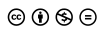
\includegraphics[height=20mm]{images/logo_cc.pdf}
%\includegraphics[height=15mm]{logo_BMFSFJ}
%\includegraphics[height=15mm]{logo_vielfaltTutGut}
\\ \\ \\


Die 1. Auflage erschien im Neisse Verlag, Dresden 2008\\
ISBN 978-3-940310-19-4\\
www.neiseverlag.de | mail@neisseverlag.de\\ \\

Lektorat: Luise Träger\\
Gestaltung und Satz: Niels Seidel / \LaTeX\\
Titelbild: Selbstportrait von Ben Mącznik aus dem Privatbesitz seines Sohnes Samson Munn.\\ \\
%Druck: Wroc\l awska Drukarnia Naukowa, PAN Wroc\l aw

}
\normalsize
\newpage
\pagestyle{plain}
\setcounter{page}{5}
\tableofcontents
\newpage


%%%%
\input{chapter/010-intro.tex}

%%%%
%\chapter{Das KZ-Außenlager Görlitz}
\input{chapter/020-goerlitz.tex}

%%%%
%\chapter{Evakuierung nach Rennersdorf und Befreiung in Görlitz}
\chapter{Evakuierung nach Rennersdorf und Befreiung in Görlitz}

Der Begriff des \glqq Todesmarsches\grqq~ist keine Wortschöpfung der Historiker, sondern von den Häftlingen der Konzentrationslager geprägt worden. Darunter verstehen sich erzwungene Märsche bewachter Gefangenenkolonnen über längere Distanzen und unter schlechten Bedingungen, in deren Verlauf viele der Häftlinge brutal gefoltert und ermordet wurden\footnote{Israel Gutman: Enzyclopädie des Holocaust, Band 3, S. 1412.}. Insbesondere in der Endphase des Krieges, als sich die alliierten Armeen den Lagern bedrohlich näherten, stellten viele Konzentrationslager ihre Funktion ein und \glqq evakuierten\grqq~die Gefangenen in andere Lager. Nicht um deren Leben willen, sondern um deren Arbeitskraft für die deutsche Kriegswirtschaft weiter ausbeuten zu können. Der Begriff der \glqq Evakuierung\grqq~kann in diesem Zusammenhang auch als verleumderischer Ausdruck dem \glqq SS-Jargon\grqq~zugeschrieben werden, da die SS sich der Tatsache bewusst gewesen sein muss, nicht nur Bewohner eines Gebietes an einen anderen Ort zu schaffen, sondern damit das Leben der Gefangenen zu riskieren. Einige Evakuierungen erfolgten auch mit der Eisenbahn, doch im Fall Görlitz wird im Folgenden klar, dass die Situation im Februar 1945 dies nicht zugelassen hätte.\newline
Genau wie die Evakuierung der Konzentrationslager, wurde auch die Evakuierung der deutschen Bevölkerung durch die Operationen der sowjetischen Armee in Schlesien diktiert\footnote{Alfred Konieczny: Groß-Rosen\index{o}{Groß-Rosen}, S. 18.}.\glqq Nun, nachdem schlagartig alle Einwohner Schlesiens, sofern sie noch zu Hause waren (d.h. im Wesentlichen: Frauen, Kinder, Alte, Kranke, Krüppel, Strafgefangene und KZ-Insassen), in Schnee und Kälte (-20 Grad Celsius) über Görlitz nach Westen drängen, ergreift uns der Strudel selbst.\grqq, schrieb ein Görlitzer Pfarrer\index{p}{Scholz, Franz}\footnote{Gemeint ist niemand geringeres als Franz Scholz, der katholische Geistliche im Görlitzer Ostteil, der über diese Zeit hinweg umfangreiche Eintragungen in sein Tagebuch machte. Später erklärte man ihn zum Ehrenbürger der Stadt Görlitz. Vgl. Franz Scholz: Görlitzer Tagebuch, 2. Auflage, S. 16.} am 11. Februar in sein Tagebuch. 
Der Historiker Alfred Konieczny gliedert die Evakuierung der schlesischen KZ-Außenlager in drei Etappen\footnote{Vgl. Alfred Konieczny: Groß-Rosen, S. 18.}. Jede dieser Etappen wirkte sich auf eine andere Art verheerend auf die Situation der Häftlinge im KZ-Außenlager Görlitz aus. In der ersten Etappe funktioniert das KZ-Außenlager als Durchgangs- und Auffanglager anderer evakuierter Lager. In der zweiten Etappe wird das Lager selbst evakuiert -- in ein provisorisches Lager im 35\,km entfernten Rennersodrf. Die dritte Etappe ist jedoch einmalig im Vergleich zu anderen Groß-Rosen\index{o}{Groß-Rosen}er Außenlagern. Die Häftlinge müssen zurück nach Görlitz und werden gezwungen, die Stadt als Festung auszubauen. 



%%%%%%%%%%%%%%%%%%%%%%%%%%%%%%%%%%%%%%%%%%%%%%%%
\section{Das KZ-Außenlager Görlitz als Durchgangs- und Auffanglager anderer evakuierter Lager}

Diese von Alfred Konieczny\label{eva_2} beschriebene Etappe war die Folge der Annäherung der Roten Armee an die Oderlinie während der zweiten Januarhälfte 1945. Seit dem 27. Januar war das KZ Auschwitz\index{o}{Auschwitz} bereits befreit, die meisten Häftlinge jedoch vorher noch auf andere Konzentrationslager, insbesondere Groß-Rosen\index{o}{Groß-Rosen}, verteilt worden. Ende Januar, so heißt es in einem Bericht eines ehemaligen Görlitzer Insassen, quartierte man Häftlinge aus Auschwitz\index{o}{Auschwitz} für eine Nacht im Lager Görlitz ein\footnote{Samuel Reifer. ZIH 301/2311.}. Ferner berichtet dieselbe Person auch von der Ankunft eines Eisenbahnwaggons mit Dokumenten aus Auschwitz\index{o}{Auschwitz}\footnote{Ebendieser. Um was für Dokumenten es sich dabei handelte und wohin sie gebracht wurden, ist ungewiss. Zeitlich spricht er vom Februar 1945. Am 12. Februar wurde Samuel Reifer, nach eigenen Angeben, ins Außenlager Zittau überstellt. ZIH 301/2311.}.
 
Alle Groß-Rosen\index{o}{Groß-Rosen}er Außenlager rechtsseitig oder unmittelbar an der Oder wurden evakuiert. Dies betraf insgesamt 11 Männer- und Frauenlager\footnote{Vgl. Alfred Konieczny: Groß-Rosen, S. 18.}.
\glqq Um den 10. Februar machte der Kommandant des Stammlagers Groß-Rosen, Johannes Hassebroek, zusammen mit dem größten Teil seines Stabes für eine Woche in Zittau Station, um sich dann in das Außenlager Reichenau im Sudetengau abzusetzen.\grqq\footnote{Dorota Sula und Andrea Rudorff: Zittau, in: Wolfgang Benz / Bar\-bara Die\-stel (Hgs.): Orte des Ter\-rors. Geschichte der nationalsozialistischen Konzentrationslager Band 6. Natzweiler. Groß-Rosen. Stutt\-hof. S. 470-473. Verlag C. H. Beck, München 2008.}~Von Zittau und später von Reichenaus aus hält Hassebroek Kontakt zu den Evakuierungsmärschen und lässt sich deren Standorte und Ausfälle durchgeben. Bereits am 15. Februar ist in einem Heeresbericht vom Frontverlauf entlang der Städte Sommerfeld\index{o}{Sommerfeld}, Sorau\index{o}{Sorau}, Bunzlau\index{o}{Bunzlau} und Goldberg\index{o}{Goldberg} die Rede. In diesem Zusammenhang ist es wahrscheinlich, dass viele Todesmärsche die Stadt Görlitz passierten und vielleicht auch im KZ-Außenlager stoppten. Hinweise darauf finden sich in Erzählungen von Leuten, die damals in der Stadt oder in der näheren Umgebung beheimatet waren\footnote{Herbert Elger sah zwischen dem 8. und 12. Februar eine Häftlingskolonne, die Görlitz in Richtung Westen verließ. Er selbst war mit einem schwer bepackten Fahrrad unterwegs und kam mehrmals mit Wächtern und Häftlingen ins Gespräch. Herbert Elger wohnte später in Stockholm. LArchB B Rep 058 Bd. 1. Franz Scholz bezeugt auch KZ-Gefangene, die Richtung Westen zogen. Vgl. Franz Scholz: Görlitzer Tagebuch, S. 16. Vgl. Siegfried Hüttig: Ortschronik Altbernsdorf.}.
Nathan Klajman\index{p}{Klajman, Nathan}, ein Gefangener des Außenlagers Kittlitztreben\index{o}{Kittlitztreben} (Trzebień, Polen), bestätigt diese Vermutung ebenso, wie der ehemalige Bunzlauer\index{o}{Bunzlau} KZ-Häftling Simon Schweitzer\index{p}{Schweitzer, Simon}. 
\newline
Nathan Klajman\index{p}{Klajman, Nathan}, der bereits im Görlitzer Lager der Organisation Schmelt inhaftiert war, bezeugt, dass während der Evakuierung des KZ-Außenlagers Kittlitztreben\index{o}{Kittlitztreben} eine große Zahl Kranker im Lager Görlitz zurückgelassen wurde.\newline 
In der Aussage von Nathan Klajmans\index{p}{Klajman, Nathan} heißt es:
\begin{leftbar}
Am 9. Februar 1945 wurden wir informiert, dass unser Feind (die Russen) heranzieht.
Wir wurden gezwungen, das Lager zu verlassen. Es begann eine Wanderung. Wer nicht imstande war weiter zu gehen, wurde sofort totgeschlagen. Nachts lagen wir oft im Schnee. Wir hatten keine Möglichkeit, um etwas zu essen. [...] Wir liefen durch Görlitz hindurch. 100 kranke Leute wurden im Görlitzer Lager zurückgelassen. Wir kamen nach Zittau\index{o}{Zittau}. Dort waren schon 300 Juden.\footnote{Nathan Klajman, ZIH 301/2765. Die hier gemachten Zahlenangaben konnten jedoch nicht weiter überprüft werden.}
\end{leftbar}

Die Häftlinge aus Kittliztreben\index{o}{Kittliztreben} verließen nach ein bis zwei Tagen das Lager und gingen über Dresden\index{o}{Dresden} bis nach Buchenwald\index{o}{Buchenwald}. Von den anfänglich 2000 Gefangenen sollen nur 360 überlebt haben\footnote{Telefonisches Interview mit Monik Mlynarski vom 18.11.2004.}.
\newline
Simon Schweitzer\index{p}{Schweitzer, Simon} schreibt, dass er Mitte Februar 1945 mit einer Kolonne Bunzlauer\index{o}{Bunzlau} Häftlinge unter der Führung des Hauptsturmführers Michael\index{p}{Michael}\footnote{Der ehemalige Häftling Simon Schweizer berichtet, der Hauptsturmführer Michael hätte unter seinen Gefangenen ein hohes Ansehen genossen. Michales Wohnort war in Görlitz. Vor seiner Zeit als Lagerkommandand war Rittmeister in der Wehrmacht.} im Lager Görlitz eintraf. Das Groß-Rosener\index{o}{Groß-Rosen} Außenlager Bunzlau\index{o}{Bunzlau} wurde kurz nach seiner Evakuierung von den sowjetischen Truppen erobert. Nach einem mehrtägigen Marsch wollte man in Görlitz vor allem pausieren und verwundete Häftlinge medizinisch versorgen. Der Görlitzer Lagerkommandant Rechenberg\index{p}{Rechenberg, Erich} hatte darum gebeten, seine Gefangenen und Wachleute der Bunzlauer\index{o}{Bunzlau} Kolonne anzuschließen. Angesichts des miserablen gesundheitlichen Zustands der Görlitzer Häftlinge wäre es den hiesigen Lagerinsassen jedoch unmöglich gewesen, mit den wesentlich kräftigeren Häftlingen aus Bunzlau\index{o}{Bunzlau} Schritt zu halten. Michael\index{p}{Michael} lehnte Rechenbergs\index{p}{Rechenberg, Erich} Anliegen ab und verurteilte den katastrophalen Umgang mit kriegswichtigen Arbeitskräften im Lager Görlitz lautstark gegenüber dem ihm unterstellten Lagerkommandanten\footnote{Simon Schweitzer: Simons langer Weg, S. 152ff.}.
\newpage
Neben den bisher erwähnten männlichen Gefangenen, kam es im Februar 1945 auch zur Überstellung von weiteren Jüdinnen. Obwohl vielfach von inhaftierten Polinnen berichtet wird, gibt Anna Hynráková Grund zu der Annahme, dass selbige erst kurz vor der Evakuierung des gesamten Görlitzer Lagers, also wenige Tage vor dem 18. Februar 1945, eintrafen\footnote{Der Hinweis von Abram Rajchbart, nach dem auch Frauen aus dem Ghetto Litzmannstadt\index{o}{Litzmannstadt} (\L \'od\'z, Polen) zusammen mit den von dort kommenden Männern viel früher in Görlitz eintrafen, konnte nicht weiter bestätigt werden.}. Dies deckt sich mit der vielfach bestätigten Überstellung von 120--180 polnischen Frauen aus dem Frauenlager Ludwigsdorf (Bojanice, Polen)\index{o}{Ludwigsdorf}\footnote{Das Außenlager Ludwigsdorf ging aus einem Lager der Organisation Schmelt hervor. Die durchweg weiblichen Gefangenen arbeiteten für Nobel-Dynamit. Der Zeitpunkt der Überstellung ins Görlitzer Außenlager variiert in den Aussagen von Chaja Zaks, Miriam Ben Shlomo und Toska Markowicz zwischen Ende März und Anfang April 1945. LArchB: B Rep 058 2231/4, sowie Mila Weisberg und Cesia Finkel; ZIH 301/923 bzw. 301/924.}. 
\newline
Es deutet sich an, dass die Evakuierung des Lagers Görlitz und damit die zweite Etappe\footnote{Vgl. Alfred Konieczny: Groß-Rosen, S. 18.} kurz bevor stand, bzw. zu dem Zeitpunkt an einigen Orten schon begonnen hatte\footnote{Ebenda. Die Evakuierung des Stammlagers Groß-Rosen\index{o}{Groß-Rosen} setzte bereits in der zweiten Februarhälfte ein.}.

%%%%%%%%%%%%%%%%%%%%%%%%%%%%%%%%%%%%%%%%%%%%%%%%
\section{Evakuierung des Lagers}

In einem Verwaltungsbericht der Stadt Görlitz vom 18. Ferbuar 1945 heißt es: \glqq Die Lage ist so kritisch, dass mit Eindringen des Feindes jeden Augenblick gerechnet werden muss\grqq\footnote{RAG Verwaltungsbericht 1944/45, S. 47.}. Zu diesem Zeitpunkt waren bereits einige Besitzungen der Stadt, wie etwa die Heide und die Grube in Kohlfurt\index{o}{Kohlfurt}, von der sowjetischen Armee besetzt. Bereits am Abend des 16. Februar ereilte ein Räumungsbefehl die in der Stadt befindlichen Zivilisten. Die Gefangenen im KZ-Außenlager standen dieser Tage schon bereit zum Abmarsch\footnote{Aussage von Anna Hynráková in einem Interview am 29.03.2005 in Prag.}, bevor am Sonntag, dem 18. Februar, Kreisleiter Malitz\index{p}{Malitz, Dr. Bruno} den endgültigen Befehl zum Abmarsch erteilte\footnote{Kreisleiter Malitz stand in der Hierarchie über dem Lagerkommandanten Rechenberg. Ungewiss ist, inwieweit die Kommandantur des KZ Groß-Rosen\index{o}{Groß-Rosen} und die WUMAG einen Einfluss auf die Evakuierung ausgeübt haben.}. Sinngemäß ließ der Lagerführer\index{p}{Zunker, Winfried} gegenüber den Häftlingen verlauteten: \glqq Da ihr als Feinde des Volkes in der Stadt Görlitz unerwünscht seid, müssen wir die Stadt verlassen\grqq\footnote{Janusch Oborowicz. BStU MfS ASt 13/48 Bd. 2 / 392.}. Gerhard Anton Sedlak\index{p}{Sedlak, Gerhard Anton}, der Fuhrparkleiter der WUMAG im Biesnitzer Grund\footnote{\glqq Im Jahre 1945 übernahm ich in dem Arbeitslager Biesnitzer Grund den Fuhrpark der WUMAG, der sich im Lager Biesnitzer Grund befand. Mir unterstanden 11 Pferde und drei paar Ochsen und ca. 10 Fuhrwerke. Außerdem war ich verantwortlich für die Verwaltung der Futtermittel, Geschirre und das gesamte Inventar. Arbeitskräfte aus dem Arbeitslager Biesnitzer Grund wurden mir für meine Arbeit nicht zugeteilt ...\grqq. Aussage von Gerhard Anton Sedlak, 1913 in Nieder Gurig, Kreis Bautzen geboren. BStU MfS ASt 13/48 Bd. 2 / 389.}, erinnert sich dessen:

\begin{leftbar} 
Während der Räumung des Lagers Biesnitzer Grund durch die Häftlinge im Februar 1945 befand ich mich in dem Fuhrpark und hörte von dort aus wiederholt Schüsse. Nachdem das Groß [im Sinne von: der Großteil] abgezogen war, ging ich durch das Lager und stellte fest, dass mehrere Häftlinge teils erschossen, teils aus anderen Ursachen -- anscheinend an Schwäche -- verstorben auf dem Erdboden lagen. Ich persönlich kann mich heute an 10--12 Leichen erinnern, die ich hier vorfand. [...] Außerdem fanden sich weitere schwache, noch lebende Häftlinge im Lager, die sich gegenseitig um Hilfe anflehten. Ich selbst traute mich nicht, ihnen Hilfe zu gewähren, weil ich damit rechnen musste, dass die zum Nachkommando gehörenden SS-Leute mich im Falle der Hilfeleistung erschießen würden.
\end{leftbar} 

Bereits am 12. Februar wurden etwa 100 kranke Gefangene ins Nebenlager Zittau\index{o}{Zittau} überstellt\footnote{Samuel Reifer wurde dann im Zittauer\index{o}{Zittau} Krankenhaus von der Roten Armee befreit. ZIH 301/2311.}. Weitere gehunfähigen Menschen blieben zunächst im Lager zurück\footnote{Im Lager Görlitz wurden etwa 200 Kranke zurückgelassen. Vgl. Jakob Rosenbaum: Von Görlitz nach Tirol, S. 39-45.}, ebenso jene für den Lagerbetrieb unabdingbare Häftlinge, wie z.B. dem Arzt Jakob Kinrus\index{p}{Kinrus, Dr. Jakob} oder dem Elektriker Jechiel Rappaport\index{p}{Rappaport, Jechiel}\footnote{Aussage von Jechiel Rappaport. LArchB B Rep 058 Bd. 2.}. Insofern kann davon ausgegangen werden, dass man mit der Evakuierung nicht beabsichtigte, die Stadt \glqq judenrein\grqq~zu machen, sondern lediglich darauf bedacht war, die Arbeitskräfte an einem sicheren Ort zu verwahren und bei Bedarf zurück zu holen. Die Tatsache, dass die Gefangenen im nur vier Kilometer entfernten Kunnerwitz mehrere Tage verweilten, spricht für diese Vermutung. Offenbar waren die Entscheidungsträger fest davon überzeugt, die Stadt Görlitz auf lange Sicht zu verteidigen und die Rote Armee weiter zurückzudrängen. Ohne diesen Gedanken vom Endsieg und der wirklichkeitsfremden Vorstellung sich als Festungsstadt behaupten zu können, hätte das Schicksal der zurückgelassenen Kranken ebenso Erschießung durch die SS oder Befreiung durch die Rote Armee heißen können. 
\newline~
\begin{leftbar} 
[Der Lagerälteste] Czech\index{p}{Czech, Hermann} befahl [...] den zum Bleiben bestimmten Personen, den anderen ihre Holzschuhe zu geben. Er befahl den Kranken auch, ihre Mäntel und Decken abzugeben.\footnote{Schlomo Graber: Schlajme.}
\end{leftbar}

\begin{leftbar}
Zuerst verließen lange Frauenreihen, und hinter ihnen Männerreihen, die Lagertore.\newline
Es begann ein Ereignis von kurzer Dauer, das zu den dramatischsten in meinem Lagerleben zählt. Auf den Landstraßen und auf den wenig benutzten Wegen schleppten wir uns unter Aufsicht der SS-Männer Richtung Osten. Der Winter war diesmal nicht streng, aber in den dünnen Sträflingsanzügen froren und zitterten wir, da es Schneeregen gab und wir mit Holzschuhen durch den kalten Matsch liefen. Ich ging eingekuschelt in einer kaputten Pferdedecke, die von einer Pritsche herunter genommen wurde. Jeder Gefangene versuchte sich etwas zu besorgen, in diesem Moment wurden die Vorschriften nicht von der Eskorte vorgeschrieben. Meine Füße waren mit Lappen umwickelt, welcher als Fußlappen dienten. Mühelos lernte ich diese Art mir die Füße zu umwickeln; sie war besser als Vorkriegsstrumpfhosen oder Socken.\newline
Ich bemühte mich während des Gehens vorn mitzulaufen, weil hinten eine größere Gefahr bestand. Hinten gingen die Schwächeren, Kranken und Nichthinterherkommenden. Trotz ihrer Mühe wurden die Abstände immer größer, sie versuchten verzweifelt nachzukommen, riefen Kumpels, um auf sie zu warten, aber es ging nicht. Mit letzter Kraft versuchten sie aufzuholen, dabei fielen sie in den Dreck. Eskortierende Soldaten schossen ihnen mit Pfeilen in den Kopf. Unseren Weg konnte man durch die da liegende Leichen verfolgen.\footnote{Schlomo Graber: Schlajme.}
\end{leftbar}

Nach dem Abmarsch der Gefangenen kehrte Hermann Czech\index{p}{Czech, Hermann} ins Lager zurück, um einige Kranke nachzuholen\footnote{\glqq Ich habe am Evakuierungsmarsch von Görlitz nach Rennersdorf teilgenommen. Ich bin aber nicht mit den gesunden Lagerinsassen gegangen, sondern mit einer kleineren Gruppe, die erst nachträglich vor dem Revier formiert wurde -- und die Kolonne einholte.\grqq, heißt es in einer Aussage von Dov Bernard Levi. LArchB B Rep 058 Bd. 5.}.

Während des gesamten Marsches zogen und schoben die Gefangenen gewaltige Wagen mit sich, auf denen sich neben einigen Lebensmitteln und persönlichen Dingen der SS und Funktionshäftlinge auch die Karthoteken der Lagerinsassen befanden\footnote{Aussage von Emmrich Schiffer. LArchB B Rep 058 Bd. 5.}. Die Bewachung der Gefangenen übernahmen neben den älteren SS-Leuten auch eine Reihe ukrainischer SS-Männer. In den Verwaltungsberichten der Stadt Görlitz findet sich während der letzten Kriegsjahre ein Hinweis auf ukrainische Schutzmannschaften der Landesschützen-Polizei, die am 30. März 1944 von Sosnowitz\index{o}{Sosnowitz} mit ihren Familien nach Görlitz überstellt wurden\footnote{RAG Verwaltungsbericht 1943/44, S. 186 II.}, doch ist es nicht sicher, ob dieselben den Evakuierungsmarsch begleiteten. 

%%%%%%%%%%%%%%%%%%%%%%%%%%%%%%%%%%%%%%%%%%%%%%%%
\subsection{Der Weg des Todes}

Die Evakuierung vollzog sich innerhalb von fünf Tagen über eine Strecke von etwa 35 Kilometern (siehe Karte:~\mymapsref{wegstrecke}). Dabei machte die Marschkolonne mehrmals Station. Die erste Etappe endete im sechs Kilometer entfernten Kunnerwitz\index{o}{Kunnerwitz}. Nach dreitägigem Aufenthalt im dortigen Stadtgut setzte sich der Marsch über Pfaffendorf\index{o}{Pfaffendorf}, Friedersdorf\index{o}{Friedersdorf} und die Schenkhäuser\index{o}{Schenkhäuser} (bei Gersdorf\index{o}{Gersdorf}) nach Obersohland\index{o}{Obersohland} fort. Dort verbrachten die Häftlinge eine Nacht auf dem Göbelschen Gut, bevor sie über die zu Kemnitz\index{o}{Kemnitz} gehörenden Lehdehäuser\index{o}{Lehdehäuser} in Richtung Buschschenke\index{o}{Buschschenke} (Herwigsdorf\index{o}{Herwigsdorf}) weiter zogen. Bis dorthin läßt sich die Route durch Zeugenaussagen und Leichenfunde eindeutig nachvollziehen. Im Wald hinter der Buschschenke\index{o}{Buschschenke} liefen die Gefangenen zunächst Richtung Strahwalde\index{o}{Strahwalde} und bogen dann links nach Berthelsdorf\index{o}{Berthelsdorf} ab. 
In Berthelsdorf\index{o}{Berthelsdorf} berichten Augenzeugen, dass ein langer Zug aus dem Wald kommend durch die Kränke (Niederdorf) kam\footnote{Laut Liesbeth Sägner.} und in Richtung Rennersdorf ging.

Dennoch besteht diesbezüglich eine Ungewissheit, da mehrfach auch Häftlinge in Oberberthelsdorf\index{o}{Berthelsdorf} gesehen wurden. Dabei handelte es sich um eine kleinere Gruppe von ca. 30 Häftlingen, die über den Oberhof (Oberdorf Berthelsdorf\index{o}{Berthelsdorf}) kam\footnote{Laut Aussage von Horst Rohland, Elfriede und Bärbel Lorenz, Berthelsdorf Hauptstraße.}. Anwohner erkannten unter den Wachleuten die gebürtige Berthelsdorferin\index{o}{Berthelsdorf} Martha Jacob\index{p}{Jacob, Martha}, die damals in Görlitz wohnte. Dieselbe wurde in Görlitz zwangsverpflichtet, Gefangene aus dem Polizeigefängnis zur Arbeit zu bringen und begleitete gezwungenermaßen auch den Evakuierungsmarsch der in dem Gefängnis am Postplatz (damals Hindenburgplatz 8) inhaftierten Menschen bis zum Herrnhuter\index{o}{Herrnhut} Bahnhof\footnote{Interview vom 25.01.2005 mit der Görlitzer Jüdin Ruth Pilz, welche zusammen mit Martha Jacob diesen Weg beschritt. Frau Jacob war weder Mitglied der SS noch gewalttätig. Ruth Pilz beschreibt sie als hilfsbereite und humane Person, die sich ebenso ihrem Schicksal ergeben musste. Vgl. auch: Roland Otto: Die Verfolgung der Juden in Görlitz während der faschistischen Diktatur, S. 102ff. Weiter Informationen über diesen Todesmarsch in: Heinz Israel: Im Wandel der Zeit -- 1285--1985, Beiträge zur 700-Jahrfeier der Gemeinde Deutsch-Paulsdorf, S. 33. Deutsch-Paulsdorf 1985. }. Der Weg von Berthelsdorf\index{o}{Berthelsdorf} nach Rennersdorf führt jedoch in entgegengesetzte Richtung, weshalb Grund zu der Annahme besteht, dass es sich dabei um einen anderen Gefangenentransport gehandelt hat. Es ist nicht auszuschließen, dass es sich dabei um KZ-Gefangene handelte, die in Rennersdorf verblieben, doch wahrscheinlich war jener im Berthelsdorfer\index{o}{Berthelsdorf} Oberdorf gesehene Todesmarsch einer von vielen, dessen Ursprung und Ziel sich heute nicht mehr bestimmen lässt. Gleiches gilt auch für den vom Altbernsdorfer\index{o}{Altbernsdorf} Ortschronist Siegfried Hüttig\index{p}{Hüttig, Siegfried} am 14.02.1945 in Altbernsdorf\index{o}{Altbernsdorf} gesehenen Marsch\footnote{Vgl. Siegfried Hüttig: 750 Jahre Altbernsdorf auf dem Eigen, S. 54.}, der entgegen vielfachen Behauptungen nicht nach Rennersdorf führte.


\mymapfigure[wegstrecke]{map_tm}{}{Wegstrecke des Todesmarsches}{Todesmarsch}{0}{}

%%%%%%%%%%%%%%%%%%%%%%%%%%%%%%%%%%%%%%%%%%%%%%%%
\subsection{Zeitzeugenaussagen}
Zeitzeugenaussagen stellen subjektive Aussagen dar, die nicht unbedingt von anderen Zeugen geteilt werden. In Bezug auf den Todesmarsch zwischen Görlitz und Rennersdorf zeigt sich dies in zum Teil widersprüchlichen und lückenhaften Berichten.   
Dennoch bilden die folgenden mündlichen oder schriftlichen Überlieferungen aus erster Hand den wertvollsten Fundus zur Rekonstruktion der Geschenisse. Der Autor möchte sich nicht anmaßen, die Gräueltaten während des Marsches mit eigenen Worten zu beschreiben, zumal sich selbst einige der befragten und unmittelbar betroffenen Personen selbst nicht im Stande sahen, das Erlebte wiederzugeben. 
~\newline
Samuel Mandelbaum\index{p}{Mandelbaum, Samuel}:
\begin{leftbar}   
 Die Leichen blieben auf der Straße liegen, die SS war aufgrund der Feindannäherung sehr nervös. Für Übernachtung und Verpflegung war keine Vorsorge getroffen worden.\footnote{Aussage von Samuel Mandelbaum. LArchB B Rep 058 Bd. 2.}
\end{leftbar}

%%%%%%%%%%%%%%%%
\paragraph{Kunnerwitz\index{o}{Kunnerwitz}}
~\newline
Wachmänner wurden damit beauftragt in Kunnerwitz\index{o}{Kunnerwitz} ein Quartier vorzubereiten\footnote{Erich Kotter erhielt von Feldfebel Homelius\index{p}{Homilius} den Auftrag dazu. BStU MfS ASt 13/48 Bd. 2 / 409.}.

Der Wachmann Erich Kotter\index{p}{Kotter, Erich} gestand nach dem Krieg ein:
\begin{leftbar}   
Beim Eintreffen am Ort ihrer Unterkunft wurden sie durch die Kapos wie das Vieh in die Ställe und Scheunen hinein getrieben und in der gleichen Art auch während ihres Aufenthaltes behandelt.\footnote{Erich Kotter. BStU MfS ASt 13/48 Bd. 2 / 409.}
\end{leftbar}

Schlomo Graber\index{p}{Graber, Schlomo}:
\begin{leftbar} 
Nach einem Marsch von sechs Kilometern -- für uns eine schier endlose Entfernung -- gelangten wir zu einem Bauernhof in Kunnerwitz\index{o}{Kunnerwitz}. Wir wurden im Pferdestall untergebracht. Auf dem Gelände fanden wir Zuckerrüben in der gefrorenen Erde. Wir fertigten provisorische Grabstöcke, mit deren Hilfe wir die Rüben ausgruben. Das war die einzige Nahrung, die uns nach zwei Tagen über die Lippen kam. Die Rüben verursachten Sodbrennen im Hals. Das aus dem Lager mitgebrachte Brot hatten sich die Blockältesten und die Kapos genehmigt.\footnote{Schlomo Graber: Schlajme, S. 85}
\end{leftbar}


Janusch Oborowicz\index{p}{Oborowicz, Janusch} berichtet ferner, dass ein entflohener polnischer Häftling am Fuße der Görlitzer Landeskrone durch Zunker am Tage des Weitermarsches erschossen wurde\footnote{Janusch Oborowicz. BStU MfS ASt 13/48 Bd. 2 / 392.}.

Janusch Oborowicz\index{p}{Oborowicz, Janusch}:
\begin{leftbar}   
Vor dem Abmarsch aus Kunnerwitz\index{o}{Kunnerwitz} erwies sich eine weitere Anzahl an Häftlingen vor Erschöpfung und wegen Krankheit gehunfähig. Wie mir später von denjenigen Häftlingen, die dem Aufräumkommando angehört hatten, erzählt wurde, sind diese gehunfähigen Häftlinge auf dem Gut Kunnerwitz\index{o}{Kunnerwitz} erschossen und in der ehemaligen Latrinengrube verscharrt worden.\footnote{Janusch Oborowicz. BStU MfS ASt 13/48 Bd. 2 / 393.}
\end{leftbar}

Nach dem Krieg fand man 13 Leichen in einer von Kompost überdeckten Latrine. Vier weitere Tote wurden an der Gutsmauer geborgen (siehe S.~\pageref{kunnerwitz}).
Der ehemalige Gefangene Israel Braun äußerte dazu:
\begin{leftbar}   
Jeden Morgen nach einer Rast musste ein Aufräumkommando, vielleicht 20 Mann, zurückbleiben und unter Leitung eines oder mehrerer SS-Männer das Rastgelände sauber machen. Stets gab es kranke oder gestorbene Häftlinge, die nicht weiter konnten. Einmal bat ein kranker Häftling, als ich zu solch einem Kommando eingeteilt war, ich sollte die Wachen veranlassen, ihn zu erschießen. Er könne nicht mehr. Er sprach nur noch mit leiser Stimme und machte den Eindruck eines Sterbenden. Der Name von ihm war Ehrenberg\index{p}{Ehrenberg}. Der SS-Mann, ich denke, es war ein Ukrainer, antwortete mir: \glqq Dieses Schwein ist die Kugel nicht wert.\grqq~Wir mussten ihn begraben, und ich denke, er hat noch gelebt.\footnote{Aussage von Israel Braun. LArchB B Rep 058 Bd. 6.}
\end{leftbar}


%%%%%%%%%%%%%%%%
\paragraph{Sohland am Rotstein\index{o}{Obersohland}}
~\newline
Etwas abseits der eigentlichen Marschstrecke, in Obersohland\index{o}{Obersohland}, machte die Kolonne ein zweites mal Station. Auf dem Gut der Familie Göbel\index{p}{Göbel} quartierte sich die SS im Wohnhaus des Bauern ein, die Häftlinge wurden in die Stallungen (siehe Bild ~\mypicsref{goebelscheune}) gesperrt. Bauer Göbel\index{p}{Göbel} war damit nicht gerade einverstanden, doch konnte er sich auch nicht dagegen wehren. Er wollte nichts mit der Sache zu tun haben und bestand deshalb unbedingt darauf, dass sein Hof nachher wieder in einem ordentlichen und sauberen Zustand gebracht wurde. Ausdrücklich verbot er der SS, Leichen auf seinen Wiesen und Feldern zu verscharren. Aufgrund dieser Auseinandersetzung holte die Gestapo Herrn Göbel\index{p}{Göbel} zu Hause ab, um ihn einem Verhör zu unterziehen. 

Janusch Oborowicz\index{p}{Oborowicz, Janusch}:
\begin{leftbar}   
Nach Kunnerwitz\index{o}{Kunnerwitz} wurde der zweite Aufenthalt in Sohland am Rotstein\index{o}{Obersohland} genommen, wo uns an Verpflegung drei Pellkartoffeln verabreicht wurden. Nach der Ausgabe eines Löffels Gemüsesalat am Tage unseres Abmarsches erhielten wir bis zu unserem Eintreffen in Rennersdorf keine weitere Verpflegung.\footnote{Janusch Oborowicz. BStU MfS ASt 13/48 Bd. 2 / 393. }
\end{leftbar}
Israel Braun\index{p}{Braun, Israel}:
\begin{leftbar}   
Auf dem Marsch gab es kaum Lebensmittel. Einmal wurde aus einem Fass löffelweise eine Art Salat an die Häftlinge verteilt. Das Fass musste man wohl gefunden haben. Nach dem Genuss dieses Zeugs erkrankten viele Häftlinge an Magenschmerzen und starben.\footnote{Aussage von Israel Braun. LArchB B Rep 058 Bd. 6.}
\end{leftbar}

\newpage
Schlomo Graber\index{p}{Graber, Schlomo}:
\begin{leftbar}   
Wir marschierten weiter über die Ortschaften Friedersdorf\index{o}{Friedersdorf} nach Sohland\index{o}{Obersohland}. Auch in diesem Dorf wurden wir im Pferdestall eines Bauernhofes untergebracht. Der Ort bot ein wenig Schutz vor der schlimmen Kälte. Wir lagen auf dem Stroh, auf dem Heuboden über uns lagerten die Frauen. Auch hier ernährten wir uns von Zuckerrüben, die wir mit Glasscherben aus der Erde gruben, und von Suppe, die wir aus Wildkräutern kochten. [...] Etwa 15 Häftlinge blieben zurück, um den Hof zu säubern. Sie stießen ein paar Stunden später wieder zu uns. Wir mussten zum Appell antreten.\footnote{Schlomo Graber: Schlajme, S. 86.}
\end{leftbar}


\begin{figure}[htb]
    \includegraphics[width=\linewidth]{images/tm_goebel.jpg}
    \caption[Göbel's Scheune in Obersohland]{Stallung auf dem Göbelschen\protect\index{p}{Göbel} Gut in Obersohland\protect\index{o}{Obersohland}}
    \label{goebelscheune}
\end{figure}

Jakob\label{rosenbaum} Rosenbaum\index{p}{Rosenbaum, Jakob}:
\begin{leftbar}   
Vor dem Abmarsch in Obersohland\index{o}{Obersohland} fragte man beim Appell, wer von den Häftlingen nicht mehr gehen konnte. Daraufhin traten neun Leute heraus.
Vor dem Abmarsch hatte man ein Kommando von 15 Männern gewählt, die den Platz reinigen sollten, wo die Häftlinge sich aufgehalten haben. [...] Ich hatte damit gerechnet, dass, wenn wir die Arbeit beendigen werden, wird der Bauer, der Eigentümer der Scheune, uns etwas geben. Als wir die Arbeit beendet hatten, waren schon Fuhrwerke vorbereitet und die ukrainischen Posten haben befohlen, die neun Gehunfähigen auf das Fuhrwerk zu setzen. Wir haben sie aufgesetzt und außerdem zwei Tote, die vor dem Abmarsch gestorben waren. Ein Ukrainer hat dem Fuhrmann befohlen, abzufahren. Auf das zweite Fuhrwerk hat er befohlen, Schaufeln und Kreuzhacken zu legen. Wir haben sofort verstanden, was das bedeutet. Wir sind dem Fuhrwerk nachgegangen. Es war mir so finster vor Augen, dass ich kaum wusste wo ich hingehe. Auf dem ersten Fuhrwerk waren Menschen aus \L \'od\'z: mein Cousin Silberberg\index{p}{Silberberg}, an den Namen des zweiten erinnere ich mich nicht, mir scheint Rosenberg. Sein Schwager, Friede hieß er, war auch im Lager. Nach einer halben Stunde sind wir zu einem Wald gekommen. Das erste Fuhrwerk mit den Menschen war schon da. Die Ukrainer befahlen, ein Grab zu graben. Die neun Menschen, als sie das gesehen haben, sind sie in Gewein ausgebrochen. Jeder hat gebeten, dass er schon wird mit marschieren. Man soll ihm nur das Leben lassen. Mein Cousin kam zu mir mit Tränen in den Augen. 
%Die siehst Jkov von den zwei Häusern, die ich in \L \'od\'z habe, wo meine Wohnung sein wird. 
Friedes Schwager saß auf der Erde und bewegte die Lippen, die Tränen flossen ihm aus den Augen.\footnote{Jakob Rosenbaum: Von Görlitz nach Tirol, S. 39-45.}
\end{leftbar}
Janusch Oborowicz\index{p}{Oborowicz, Janusch}:
\begin{leftbar}   
Erschöpfte und kranke Häftlinge, die von Sohland\index{o}{Obersohland} aus den Marsch nicht fortsetzen konnten, jedoch andererseits mit eigenen Augen gesehen hatten, was ihren Leidensgenossen passierte, hatten sich vor dem Abmarsch in der Scheune versteckt. Der Bauer Göbel, bei dem wir untergebracht waren, hatte dies jedoch beobachtet und machte die Wachmannschaft darauf aufmerksam, worauf eine Durchsuchung der Scheune erfolgte. Die hierbei vorgefundenen Häftlinge wurden am nächsten Waldrand von der SS-Wachmannschaft erschossen.\footnote{Janusch Oborowicz. BStU MfS ASt 13/48 Bd. 2 / 393. }
\end{leftbar}

Janek Schilid\index{p}{Schilid, Janek} berichtet übereinstimmend:
\begin{leftbar}
Mit einem vom Bauer Göbel\index{p}{Göbel} zur Verfügung gestellten Fuhrwerk wurden die Häftlinge an den nächsten Waldrand gefahren, dort vom Wagen herunter geholt und von Angehörigen des Wachpersonals erschossen.\footnote{Janek Schilid, am 04.08.1914 in Jaloschin/Welonyen geboren. BStU MfS ASt 13/48 Bd. 2 / 397.}
\end{leftbar}

\newpage
%%%%%%%%%%%%%%%%
\paragraph{Lehdehäuser}
Ein Mann aus den Lehdehäuser\index{o}{Lehdehäuser}n, der nicht namentlich genannt werden möchte, sah die Häftlingskolonne am elterlichen Haus vorbeiziehen:
\begin{leftbar} 
Zusammen mit meinem kleineren Bruder beobachteten wir vorbeiziehende Häftlinge. Sie trugen längs gestreifte Kleider und eine kleine Mütze. Viele liefen barfuß, die anderen hatten sich Lumpen um die Füße gebunden. Durchweg allen konnte man ihre widrige Versorgungslage ansehen, ihre Gesichter waren eingefallen und zeugten von Unterernährung. Inmitten der Kolonne wurden mehrere großrädrige Bauernwagen, die lediglich mit Brettern belegt waren, gezogen. Ein jeder dieser zwei mal vier Meter großen Wagen wurde durch ca. 20 Häftlinge an zwei Seilen gezogen und von allen Seiten geschoben. Die Wagen waren für die Leichen sowie Grabwerkzeuge bestimmt. Der Zug wurde im Abstand von 30 Metern von SS-Wachleuten begleitet.\newline
Einige Häuser zuvor hatte Frau Talke\index{p}{Talke} einen Viertelkorb Äpfel auf die Straße geschüttet, damit sie sich die Gefangenen greifen konnten. Vor dem Haus meiner Eltern stand ein Brunnen, an dem einige Häftlinge den Schwängel betätigten, um Wasser hochzupumpen. Die SS-Wachleute ließen dies nicht zu und schlugen mit ihren Gewehrkolben auf die Dürstenden ein. Ein Häftling brach, nachdem er am Haus vorbei gelaufen war, auf der Straße zusammen. Sogleich stieß ihm ein Wachmann sein Knie in den Rücken, so dass er ganz zu Boden sank und durch einen Genickschuss getötet wurde. Ihn haben sie auf einen der Wagen geladen. Ehe alle Häftlingen an den Lehdehäuser\index{o}{Lehdehäuser}n vorbeigezogen waren, verging einige Zeit, doch viel länger dauerte es, bis das Gewehrfeuer in der Ferne verstummte.\footnote{Interview vom 16.10.2004 in den Lehdehäuser\index{o}{Lehdehäuser}n / Kemnitz.}
\end{leftbar}

Im Prozess gegen Zunker und Czech gab ein Zeuge zu Protokoll:
\begin{leftbar}   
Josef Bursztyn\index{p}{Bursztyn, Josef} war während Evakuierung so schwach geworden, dass er nicht mehr weiter gehen konnte und sich auf den Boden setzte. Zunker ging auf ihn drauf zu und forderte ihn auf, aufzustehen, worauf er Zunker bat, ihn doch zu erschießen, damit seine Qualen ein Ende haben. Zunker befahl zwei anderen Häftlingen, ihm aufzuhelfen und erschoss ihn dann.\footnote{Prozessakten von Czech. LArchB B Rep 058 Bd. 2.}
\end{leftbar}

%%%%%%%%%%%%%%%%
\paragraph{Buschschenke}
~\newline
Gerda Bötig\index{p}{Böetig, Gerda} erinnert sich heute mit Schrecken an den Todesmarsch, damals besaßen ihre Eltern die zwischen Herwigsdorf\index{o}{Buschschenke} und Kemnitz\index{o}{Kemnitz} gelegene Gastwirtschaft in der gleichnamigen Buschschenke\index{o}{Buschschenke}:
\begin{leftbar}   
Beim Eintreffen der Häftlingskolonne wollten die Gastleute den völlig ausgehungerten Gefangenen Wurstbrühe geben. Die Wachmannschaften verboten dies jedoch, und so gelang es ihnen nur, eine Wanne mit Wasser in den Hof zu stellen. Auf demselben Wege wie die Häftlingskolonne kam ich einige Zeit später aus Richtung Kemnitz\index{o}{Kemnitz} zur Buschschenke\index{o}{Buschschenke}, wo die Häftlinge bereits beim Appell standen. Etwa 100 Meter vor der Buschschenke\index{o}{Buschschenke} sah ich einen Häftling auf der Straße liegen, der vor Erschöpfung nicht mehr weiter konnte. Ich erzählte dies den SS Bewachern in der Hoffnung, dass diese dem Häftling helfen und ihn nachholen. Diese taten nicht dergleichen und entgegneten mir stattdessen: \glqq Wir machen ihn fertig\grqq.
Kurz darauf wurde der Häftling erschossen. Die Opfer zogen sie in einem Karren hinterher. Der Todesmarsch setzte sich in Richtung Strahwalde\index{o}{Strahwalde} fort.\footnote{Interview mit Gerda Bötig durch Kurt Wolf vom Sommer 2004.}
\end{leftbar}

Jakob Rosenbaum\index{p}{Rosenbaum, Jakob}: 
\begin{leftbar}   
Wir gehen weiter, wir treten auf Tote. Wir bemerken, wie im Wald ein paar Menschen sitzen. Ich schreie steht auf! Ich habe gar nicht bemerkt, dass zwei Soldaten sie bewachen und Menschen schon ein Grab graben. Als wir uns etwas entfernt haben, hörten wir eine Schießerei. Wir gehen den Weg weiter, der nach Reichenbach führt. Nach einem ganzen Tag Marschieren, sind wir in Regersdorf [gemeint ist Rennersdorf] stehen geblieben.\footnote{Jakob Rosenbaum: Von Görlitz nach Tirol, S. 39-45.}
\end{leftbar}

Am selben Weg endeckten Waldarbeiter nach dem Krieg eine mit Reisig verdeckte Grube. Unter den Zweigen lagen sieben Leichen (siehe Ermittlungen gegen die NS-Verbrechen S.~\pageref{buschschenke}).

\begin{leftbar}   
Auf dem Wege haben wir viele Tote gesehen. Ich habe unter anderem den Juden Rosensaft\index{p}{Rosensaft} aus \L \'od\'z\index{o}{Litzmannstadt} gesehen. Das Blut ist ihm aus dem Mund gerinnt. Ich habe mich ihm genähert und versucht ihn aufzustellen. Er hat mit der Hand eine Bewegung gemacht und gemeint: Rosenbojm, lass mich sterben. Ich wollte ihm erzählen, was im Wald passierte, in diesem Moment ist der Rapportführer gekommen und hat ihn erschossen.\footnote{Jakob Rosenbaum: Von Görlitz nach Tirol, S. 39-45.}
\end{leftbar}

%%%%%%%%%%%%%%%%
\paragraph{Rennersdorf}
~\newline
Am Nachmittag des 23. Februar 1945 erreichten die Häftlinge die Ortschaft Rennersdorf. 

Janusch Oborowicz\index{p}{Oborowicz, Janusch}:
\begin{leftbar}   
Nach Sohland\index{o}{Obersohland} galt als nächstes Ziel Rennersdorf, wo wir in den späten Abendstunden eintrafen. Noch wenige 100 Meter vor dem Ziel fielen einige Häftlinge vor Erschöpfung um, die dann sofort an der Straße von den Angehörigen des Wachpersonals erschossen wurden.\footnote{Janusch Oborowicz, am 25.05.1923 in Breslau geboren. BStU MfS ASt 13/48 Bd. 2 / 393.}
\end{leftbar}

Frau Liesbeth Sägner\index{p}{Sägner, Liesbeth} beobachtete im Alter von 11 Jahren die vorbeiziehenden Häftlinge:
\begin{leftbar}   
Sie waren gehüllt in Sträflingskleidung und Lumpen. Sie liefen in Zweierreihen und bildeten eine lange Kette mit vielen Unterbrechungen. Wachleute begleiteten den Zug mit ihren großen Hunden.\footnote{Liesbeth Sägner während eines Interviews in Rennersdorf, 2005.}
\end{leftbar}

Die Rennersdorferin Hildegard Fleischmann\index{p}{Fleischmann, Hildegard}:
\begin{leftbar}   
Ich befand mich seinerzeit vor der Seliger-Schmiede\index{p}{Seliger} und beobachtete, wie einer der Häftlinge vor Erschöpfung zusammenbrach. Hierauf trat ein Angehöriger des SS-Wachpersonals an den Zusammengebrochenen heran und versuchte ihn mit den Füßen in den neben der Straße fließenden Bach zu stoßen. Der Schmied Seliger\index{p}{Seliger} beobachtete gleichfalls diesen Vorfall, trat an den SS-Mann heran und sagte: \glqq Na, na, soweit ist es nicht, dass er in den Bach gekippt wird\grqq. Er bot einen Handwagen zum Abtransport des Häftlings an, womit dann der zusammengebrochene Häftling mit einem zweiten Juden, der bereits einige Zeit vorher zusammengebrochen war, weggefahren wurde.\footnote{Hildegard Fleischmann, am 02.09.1915 in Schlegel geboren. BStU MfS ASt 13/48 Bd. 2 / 460. Bestätigt wurde dies auch durch Liesbeth Sägner während eines Interviews in Rennersdorf. Auch Christa Schuberts Großmutter hat dies gesehen.}
\end{leftbar}

Die damalige Rennersdorferin Christa Schubert\index{p}{Schubert, Christa} entsinnt sich der Schrecken des 23. Februar 1945, dem Tag ihres 12. Geburtstags:

\begin{leftbar}   
Unsere Großmutter kam aus dem Oberdorf und hat sie [die Häftlinge] gesehen. Wenn sie von Berthelsdorf\index{o}{Berthelsdorf} kommen, bei der ersten Wirtschaft. Dort hat unsere Großmutter gewohnt. Und wir haben unten bei Schulzes Brücke [Abzweig Herrnhut] gewohnt und sie wollte zum Kaffee trinken zu meinem 12. Geburtstag runter kommen, da hat sie das schon von dort oben gesehen. Sie konnte sich noch erinnern, dass bei der Seliger-Schmiede, wo jetzt Bachmanns wohnen, einige nicht mehr richtig fort konnten. Dort musste der Schmied einen Leiterwagen geben. [...] Die Großmutter sah zu, dass sie weg kam. Der Zug ist dann hinterher gekommen. Das ist nach dem Mittag gewesen, denn da war ja überall Landwirtschaft, und das Vieh war zu füttern, deshalb musste in der dritten Stunde Kaffee getrunken werden. Wir haben in der Küche auf der Bank gestanden und zum Fenster raus geguckt. Ich kann mich noch genau entsinnen, weil da ein Zweiräder [Wagen] war und die Köpfe auf der Straße hingen und schleiften. Das war furchtbar. Die hatten solche großen Wagen und dort lagen Menschen drauf. Den haben die Gefangenen vorn gezogen und darauf lagen die, die nicht mehr fort konnten. Die waren furchtbar angezogen, die Sachen hingen so runter und es war ja Winter.
Mein Vater, meine Mutter auch, jeder war entsetzt; auf so etwas war ja niemand gefasst.\footnote{Interview mit Christa Schubert, Berthelsdorf, den 01.04.2005.}
\end{leftbar}

\section{Das Ausweichlager Rennersdorf}

Die Überlebenden des Todesmarsches kamen am 23. Februar in das unweit von Herrnhut\index{o}{Herrnhut} gelegene Rennersdorf. Die SS quartierte die Häftling in einem alten herrschaftlichen Gutshof am Fuße des Berges Eichler ein.
Das sogenannte Gut Oberrennersdorf (Bild ~\mypicsref{gutoberrennersdorf}) befand sich seit 1765 im Besitz der Brüder-Unität Herrnhut\index{o}{Herrnhut}.
Unter dem Vorwand der Knappheit von Siedlungsland und der strategischen Lage in Grenz\-nähe zur Tschechoslowakischen Republik erwirkte die Wehrmacht nach zähen Verhandlungen den Verkauf des Gutes Oberrennersdorf als Bestandteil des Remonteamtes (zusammen mit dem Berthelsdorfer\index{o}{Berthelsdorf} und Großhennersdorfer Gut) am 3. März des Jahres 1937\footnote{UArch 7275.}. Dem damaligen Pächter Rosenberg wurde im Juli des selben Jahres gekündigt\footnote{Ebenda}. 
Das tote wie auch das benötigte lebende Inventar ging in den Besitz der Wehrmacht über. Die landwirtschaftlichen und forstwirtschaftlichen Unternehmungen setzte man fort, wobei die Pferdeaufzucht eine wesentliche Rolle spielte. 
Laut dem Rennerdorfer Ortschronisten war der damalige Wirtschaftsvogt und Betriebsführer ein gewisser Reinhold Lehmann\index{p}{Lehmann, Reinhold}\footnote{Vgl. Robert Heinze: Ortschronik Rennersdorf. Reinhold Lehmann (*26.03.1889) war eines von insgesamt 60 NSDAP Mitgliedern im Ort, die im Zuge der Entnazifizierung durch die sowjetische Militärkommandantur ermittelt wurden. KArchLZ Rennersdorf / 142. }. Außer ihm wohnten noch eine Reihe anderer Personen auf dem Gut: der Tierarzt Zwerschke mit seinem Sohn, ein Schäfer namens Schlaffke sowie die Familien Bittrich, Feder, Engel und Weber. 

\paragraph{Welcher Art war das Lager in Rennersdorf?} Genau wie das hier bereits behandelte Görlitzer Lager im Biesnitzer Grund, ist das Lager in Rennersdorf definitionsgemäß kein Konzentrationslager\footnote{Im Sinne der Inspektion der Konzentrationslager von Oswald Pohl.}. Ebenso wenig kann man es als Arbeitskommando bezeichnen, da nur geringfügige Arbeitseinsätze erfolgten. 
Vielfach wurde das Lager in der Literatur als KZ-Außenlager bezeichnet, wobei es jedoch, entgegen Isabell Sprengers Annahme, kein reines Männerlager war\footnote{Vgl. Isabell Sprenger: Groß-Rosen, S. 232.}. Angesichts der Tatsache, dass die Gefangenen nur für knapp zwei Wochen in Rennersdorf verweilten und anschließend wieder an ihren Ausgangspunkt nach Görlitz zurückkehrten, scheint es im wörtlichen Sinne ein Ausweichlager gewesen zu sein. Im Archiv des KZ Groß-Rosen\index{o}{Groß-Rosen} sowie in den Verwaltungsbüchern der Gemeinde Rennersdorf existiert kein einziges Dokument, was den Zusammenhang mit dem Hauptlager erkennen lässt. Belegt ist hingegen der enge Kontakt zwischen den Kommandoführern der Evakuierungsmärsche und dem Meldekopf des Stammlagers, welcher sich ab dem 17. Februar 1945 im Außenlager Reichenau im Sudetengau (Rychnov u Jablonce nad Nisou, Tschechien)\index{o}{Reichenau} befand. 
Im Folgenden wird das Lager in Rennersdorf dennoch als KZ-Außenlager bezeichnet, um damit einerseits den Charakter eines KZ-Lagers auszudrücken und andererseits eine von der Existenzdauer unabhängige Benennung beizubehalten\footnote{Gleiches gilt für das KZ-Außenlager Kunnerwitz, wo bereits vor dem Durchmarsch der Görlitzer KZ-Häftlinge ein Groß-Rosener Arbeitskommando bestand. Sohland am Rotstein, als zweite Station während des Todesmarsches von Görlitz nach Rennersdorf, soll jedoch nicht als KZ-Außenlager angesehen werden, da die Gefangenen dort nur einen Tag verweilten und kein geordneter Lagerbetrieb errichtet bestand.}. 
%Offenbar gab es für diese einzige Einquartierung von KZ-Häftlingen eine Übereinkunft zwischen SS oder der Görlitzer Kreisleitung und der Wehrmacht als Eigentümer der Gebäude und Ländereien. 

\myfigure[gutoberrennersdorf]{renn01}{}{Das Gut Oberrennersdorf}{Gut Oberennersdorf}{0}



%%%%%%%%%%%%%%%%%%%%%%%%%%%%%%%%%%%%%%%%%%%%%%
\subsection{Die Haftbedingungen im Lager Rennersdorf}
Das Außenlager Rennersdorf hatte einen stark provisorischen Charakter und ist kurzfristig eingerichtet worden. Das Gelände war weder durch
einen Zaun gesichert, noch von der zivilen Außenwelt isoliert. Die vorherige Nutzung als Remontegestüt\footnote{Ein Remontegestüt sorgt für die Aufzucht von jungen Pferden als Ersatz für solche, die durch Krieg oder andersartig sterben.} war für die Gefangenen mehr als offensichtlich. Die Unterbringung erfolgte im 70\,m nördlich gelegenen Pferdestall (Bild ~\mypicsref{pferdestallfoto}) zwischen einem kleinen Wäldchen und dem Weg nach Neundorf.
Der Pferdestall teilt sich in vier Abschnitte. Im hinteren, vierten Abschnitt, welcher dem Gutshof am nächsten liegt, waren die Frauen untergebracht. In den anderen drei Abschnitten waren die Männer einquartiert.

% 1:label, 2:bildname, 3:fuootnote, 4:caption, 5:list_of_pics_name
\myfigure[pferdestallfoto]{renn03}{}{Der Pferdestall}{Pferdestall in Rennersdorf}{0}

Die Situation der Häftlinge war geprägt durch die gesundheitlichen Folgen des langen Marsches und die Unzulänglichkeiten des provisorischen Lagers. Beides zusammen zehrte an den physischen und mentalen Kräften der Menschen im Lager. Aufgrund der Haftbedingungen kann man, im Vergleich zum Außenlager Görlitz, nicht von einem geregelten, für fast alle geltenden Tagesablauf sprechen. 

Der ehemalige Gefangene Abram Rajchbart\index{p}{Rajchbart, Abram} drückt mit wenigen Sätzen aus, unter welchen Bedingungen die KZ-Gefangenen in Rennersdorf hausten:

\begin{leftbar} 
Hier herrscht Chaos. Wir schlafen auf dem Mist, der mit Stroh bedeckt wird. Die Lebens- und Arbeitsbedingungen sind unmenschlich und entsetzlich. Wir haben keine Möglichkeiten, uns zu waschen und die Wäsche zu wechseln. Das Ungeziefer verbreitet sich, auch die Krankheiten breiten sich aus.\footnote{Aussage von Abram Rajchbart. Jüdisch Historisches Institut Warschau, 301/715.}
\end{leftbar}

Es gab weder ein Krankenrevier noch einen Waschraum. Im Gegensatz zum Görlitzer Lager, existierte keine Wäscherei, Schusterei oder Schneiderei. Die Einrichtung des Lagers reduzierte sich auf eine Küche und eine Latrine aus Birkenholz\footnote{Laut einem Interview  mit Ilse Gießler, Dresden 2005.}. Der Pferdestall diente als \glqq Menschenstall\grqq, ohne Betten, bestenfalls mit etwas Stroh ausgelegt\footnote{Aussage von Max Wachsmann. LArchB B Rep 058 Bd. 6.}. Janusch Oborowicz führt dazu weiter aus:

\begin{leftbar} 
Infolge der in dem Pferdestall bestehenden ungünstigen hygienischen Verhältnisse, hervorgerufen durch die schlechte Luft und die Ausdünstungen des Mistes, haben sich auch die Läuse bei den Häftlingen auffallend vermehrt.\footnote{Aussage von Janusch Oborowicz. BStU MfS ASt 13/48 Bd. 2 / 392.}
\end{leftbar}




\subsection{Die Versorgungslage der Häftlinge}


Janusch Oborowicz\index{p}{Oborowicz, Janusch}:
\begin{leftbar} 
An Verpflegung erhielten wir seinerzeit für acht Häftlinge jeweils 1 Brot und 3/4 Liter halb rohe Gemüsesuppe. Neben den Erschießungen waren infolge der schlechten Ernährung auch weitere Sterbefälle zu verzeichnen.\footnote{Aussage von Janusch Oborowicz, BStU MfS ASt 13/48 Bd. 2 / 392.}
\end{leftbar}

Die Unterernährung war den Gefangenen anzusehen und äußerte sich in der verzweifelten Suche nach Nahrung. Einige der Notleidenden brachten es fertig, so Ilse Gießler\index{p}{Gießler, Ilse}, eine Scheibe Brot von der Straße aufzuheben ohne sich dabei auffällig bücken zu müssen\footnote{Interview mit Ilse Gießler, Dresden, März 2004.}. 

Die ehemalige Rennersdorferin Ilse Gießler\index{p}{Gießler, Ilse} erinnert sich:
\begin{leftbar} 
Fast täglich kamen Häftlinge an unserem Haus vorbei, um beim Bäcker Alter mit einem hierfür gebauten Spezialfahrzeug Brot als Verpflegung für die Häftlinge abzuholen. Eines Tages {[}...{]} war ich Augenzeuge, wie einer der Häftlinge während der Rückfahrt vom Bäcker zum Gute, unmittelbar vor unserem Hause, von einem Posten der SS-Mannschaft mit einem armstarken Knüppel schwer misshandelt wurde, indem er auf ihn einschlug, wobei ihn der noch anwesende Kapo zu halten hatte. Da uns einerseits verboten war, den Häftlingen irgendwelche Nahrungsmittel zu verabreichen oder gar mit ihnen zu sprechen, wir andererseits tiefstes Mitleid mit ihnen empfanden, hat mein Vater eines Tages Äpfel so in den Straßengraben geworfen, dass die Häftlinge sie auf ihrem Rückweg vom Bäcker sehen mussten, wodurch ihnen diese Zuwendung auch tatsächlich gewährt werden konnte. Das Fuhrwerk wurde tatsächlich von ca. 10\textendash{}12 Juden gezogen bzw. geschoben. Alle Häftlinge machten einen verwahrlosten und verhungerten Eindruck
\footnote{Ilse Gießler, am 24.12.1920 in Niederrennersdorf geboren. Die damals 26jährige bewohnte mit ihren Eltern ein heute nicht mehr stehendes Haus an der Hauptstraße (zwischen dem Abzweig Herrnhut und dem Wehr). Ihr Vater war vor 1933 KPD Mitglied, sie selbst ist weder dem Bund Deutscher Mädel, noch einer anderen NS-Organisation beigetreten und wurde deshalb vom damaligen Ortsgruppenleiter für \glqq vogelfrei\grqq~erklärt. Im Jahre 1948 wurde sie als Zeugin im Malitz-Meinshausen-Prozess vorgeladen, jedoch aufgrund der ausreichenden Beweislast gegen die Angeklagten nicht mehr angehört. BStU MfS ASt 13/48 Bd. 2 / 462. Interview mit Ilse Gießler, Dresden, März 2004.} 
\end{leftbar}


Während seit Ankunft der Gefangenen ihre Unterernährung für die Dorfbevölkerung nicht übersehbar war, machte die SS keinen Hehl daraus, im Überfluss zu leben. In jener Zeit hatten selbst die Leute im Dorf nicht übermäßig viel zu essen und empörten sich daher nicht ohne Grund über die Verfütterung von großen Wurstringen an die Hunde der SS\footnote{Laut Aussage mehrerer Zeitzeugen, darunter Ilse Gießler, Helmut Sperling sowie Siegfried und Wolfgang Bittrich.}. Die überschwänglichen SS-Gelage in der Schmidt-Mühle wurden mit Entsetzen durch die Bevölkerung aufgenommen.

Schlomo Graber\index{p}{Graber, Schlomo} erinnert sich der Situation in seinen Memoiren:
\begin{leftbar} 
Die Deutschen schlachteten sich Schafe, warnten uns jedoch, wer sich an den Schafen vergreife, sei des Todes. Hier teilte man uns auch je eine Scheibe Brot zu, die jeder in seinem Brotbeutel wie einen Schatz hütete, um sie krümelweise zu essen. Als ich eines morgens aufwachte -- ich lag zwischen Vater und einem anderen Juden -- spürte ich, dass dieser sich nicht mehr regte, und suchte als erstes sein Brot. Als ich es gefunden hatte, freute ich mich an dem Fund.

An jenem Morgen erschien der älteste Soldat, der die Küche der Deutschen unter sich hatte, und rief mich: \glqq Farzer komm schnell\grqq. Er forderte mich auf, den geschlachteten Schafen das Fell abzuziehen. Von ihm erfuhr ich, dass kranke Schafe für die Häftlinge gekocht werden sollten. Ich fand eine Methode die Schafe krank zu machen. Ich ging in den Pferch, trat einem Schaf in den Bauch, dass es umkippte, und erklärte: \glqq Dies ist krank\grqq. Auf diese Weise bekamen wir nach langem Hungern etwas in den Magen.\footnote{Schlomo Graber: Schlajme, S. 87.}
\end{leftbar}
Die Landarbeiterin Auguste Hergarten\index{p}{Herrgarten, Auguste}: 
\begin{leftbar} 
Die Häftlinge bekamen ein Essen, dass man nicht einmal als brauchbares Schweinefutter bezeichnen kann. Es war furchtbar mit anzusehen, wie die hilflosen armen Menschen immer wieder schwersten Mißhandlungen ausgesetzt waren. Sobald sich eine Gelegenheit bot, steckten wir ihnen zusätzlich etwas Essen zu, obgleich wir selbst nicht viel hatten.\footnote{Auguste Hergarten, am 22.06.1893 in Berthelsdorf geboren. BStU MfS ASt 13/48 Bd. 2 / 464.}
\end{leftbar}


%% Arbeit und Ernährung
Der Rennersdorfer Helmut Sperling erinnert sich, wie sein Vater bei der Lagerleitung um Hilfe beim Fällen einer Eiche bat. Seine Mutter erwartete die Helfer mit einem Teller Schnitten, welcher jedoch von den Bewachern auf dem Erdboden zertrampelt wurde.


%%%%%%%%%%%%%%%%%%%%%%%%%%%%%%%%%%%%%%%%%%%%%%
\subsection{Zwangsarbeit auf dem Gut Oberrennersdorf}
Der Bericht des Zeitzeugen Helmut Sperrling legt die Vermutung nahe, die Häftlinge seien auch in Rennersdorf von der Zwangsarbeit verschont geblieben. Dies wird jedoch in nur in sehr wenigen Überlieferungen ehemaliger Gefangener bezeugt. Ein Großteil der Menschen war nach dem anstrengenden Marsch nach Rennersdorf physisch und psychisch kaum noch in der Lage zu arbeiten. Angesichts dessen wird nur eine Minderheit, vor allem aber Frauen, zur Arbeit herangezogen worden sein\footnote{Vor und nach der Evakuierung gibt es übereinstimmende Zeugenaussagen, wonach die Frauen in einer eindeutig besseren körperlichen Verfassung waren als die Männer.}.
Die Art der Arbeit richtete sich nach den örtlichen Erfordernissen der im Hof betriebenen Landwirtschaft.
Damals arbeitete neben vielen anderen auch Liesbeth Sägners\index{p}{Sägner, Liesbeth} Mutter im Gut Oberrennersdorf als Landarbeiterin. Sie wusste zu berichten, dass die Häftlinge mit ihr und anderen Rüben sortieren mussten. Obwohl sie sich in einem erbärmlichen Zustand befanden, war es ihnen verboten von den Möhren zu essen, weshalb Frau Sägners Mutter ihnen aus Mitleid mehrmals einen Kanten Brot bei der Arbeit zuschob\footnote{Laut Liesbeth Sägner.}. 
Abram Rajchbart\index{p}{Rajchbart, Abram} beschreibt die Arbeitsbedingungen insgesamt als unmenschlich und entsetzlich\footnote{Aussage von Abram Rajchbart. ZIH 301/715.}. Die Annahme der Historiker Gräfe / Töpfer und Zg\l obicki, wonach in Rennersdorf Schanzarbeiten verrichtet wurden, konnte in den zahlreichen Überlebendenberichten nur gegenteilige Bestätigung finden, zumal es in ganz Rennersdorf keine Überreste solcherlei Arbeit gibt. Aller Wahrscheinlichkeit nach handelte es sich hierbei um eine Verwechslung mit den bei der Rückkehr nach Görlitz befohlenen Schanzarbeiten.\footnote{Vgl. Gräfe / Töpfer: Die Konzentrationslager auf dem Territorium des heutigen Sachsens. Vgl. auch: Roman Zg\l obicki: Obozy i cmentarze Wojenne w Zgorzelcu.}. 




%%%%%%%%%%%%%%%%%%%%%%%%%%%%%%%%%%%%%%%%%%%%%%
\subsection{Kontakt zur Dorfbevölkerung}
Rennersdorf hatte während des Krieges nur wenige hundert Einwohner, die fast alle miteinander bekannt waren. Die Neuigkeit von der Ankunft der erbärmlich ausschauenden Häftlinge am 23. Februar 1945 verbreitete sich also rasch, zumal die Kolonne zuvor auf gut zwei Kilometern die Hauptstraße des Ortes passierte. 

\glqq Jeder wusste es\grqq\footnote{Laut Ilse Gießler und vielen anderen teils ehemaligen Rennersdorfern.}. Die Neuigkeit von der Ankunft der erbärmlich ausschauenden Häftlinge verbreitete sich rasch. Den Pferdestall, in dem die Häftlinge untergebracht waren, konnte man sehr gut von der am Eichler vorbeiführenden Straße zwischen Herrnhut\index{o}{Herrnhut} und Bernstadt\index{o}{Bernstadt} / Großhennersdorf\index{o}{Großhennersdorf} einsehen. Ilse Gießler berichtete, wie sie während eines Waldspazierganges auf dem Berg Eichler die abgemagerten Gefangenen beobachten konnte. Insbesondere jene Rennersdorfer, die auf dem Gutshof wohnten oder arbeiteten, konnten sich der Präsenz der Gefangenen keinesfalls verschließen. Offensichtlich hielt die SS Appelle im Hof des Gutes ab, bei denen es immer wieder zu Folterungen kam\footnote{Interview mit den Brüdern Bittrich, die einst als kleine Jungen im Alter von 4 und 8 Jahren Zeuge der Gewalt wurden. Rennersdorf, 29.03.2004.}. Die SS - seit dem Todesmarsch durch eine ukrainische Einheit verstärkt - provozierte durch ihren Umgang mit den Gefangenen bei den Hofbewohnern eine Angst, selbst in Mitleidenschaft gezogen zu werden. Die Rennersdorfer sollten sehen, was ihnen blühte, wenn sie den Gefangenen Mitleid entgegen brachten.

%\begin{landscape}
\mymapfigure[karterennersdorf]{map_rennersdorf}{}{Rennersdorf}{Rennersdorf}{0}{33}%0.515
%\end{landscape}

Bereits bei der Ankunft, als die Gefangenen das Hoftor passierten, deutete sich alles an. Es kam zu einer ersten Erschießung vor den Augen einiger Frauen und Kinder. Janek Schilid  sagte 1948 dazu:

\begin{leftbar} 
Da vor dem Erreichen des Dorfes ein ziemlich steiler Berg zu überwinden war, da einer der Häftlinge zu schwach war, den sich hieraus ergebenen körperlichen Anforderungen gerecht zu werden und zusammen sank, wurde er an der Straße durch angehörige des Wachpersonals erschossen. \footnote{Janek Schilid. BStU MfS ASt 13/48 Bd. 2 / 397.}
\end{leftbar} 

%Weitere Erschießungen beobachten Kinder hinter dem Hof an einem Wiesenweg\footnote{Laut Helmut Sperling.}. Von weitem sichtbar hatte die SS an einer Linde neben dem Pferdestall einen Häftling aufgehangen\footnote{Laut Wolfgang und Siegfried Bittrich.}. 

\newpage
Die Unterernährung war den Gefangenen anzusehen und äußerte sich in der verzweifelten Suche nach Nahrung. Dabei ersuchten sie auch Rennersdorfer um Hilfe. Jedoch stets unter Gefahr, von der SS erwischt zu werden, wie jene beim Bauer Schönfelder\index{p}{Schönfelder}\footnote{Vgl. Katja Junge: Der Todesmarsch vom KZ-Außenlager Biesnitzer Grund nach Rennersdorf 1945, unveröffentlichtes Manuskript, S. 6.}.

Außerhalb des Gutshofes und bei der Abholung des Brotes beim Bäcker\index{p}{Alter} kamen die Häftlinge jedoch kaum in Kontakt mit der Dorfbevölkerung. 

%% Löwe
Bemerkenswert ist die Begegnungen im Hause der Familie Löwe, welche unweit vom SS-Quartier in der Schmidt-Mühle wohnte: Joachim Löwes Mutter war an Fieber erkrankt und man befürchtete, eine Epidemie könntex sich ausbreiten. Der Arzt im Nachbarort Herrnhut war verhindert, weshalb sich der NSDAP-Ortsgruppenleiter nach einem Arzt unter den jüdischen Häftlingen erkundigte und fündig wurde. Die Behandlung durch einen jüdischen Arzt galt in jener Zeit als \quotedblbase{}Rassenschande\textquotedblleft{}. Seit dem Erlass der Nürnberger Gesetze (15.09.1933) war es jüdischen Ärzten untersagt, \quotedblbase{}Arier\textquotedblleft{} zu behandeln. Trotzdem gestattete die Lagerleitung dem Arzt Frau Löwe zu behandeln. Mit einer Medikamententasche erschien er im Haus der Löwes. Einer der beiden ihn begleitenden Bewacher wollte zunächst der Behandlung beiwohnen, erst als Frau Löwe mit einem Fingerzeig auf das Bild ihres im Krieg gefallenen Gatten hindeutete, verließ der SS-Mann die Stube. Der Arzt war mit Medikamenten sowie notwendigen Utensilien ausgestattet und somit in der Lage der Erkrankten bei diesem und zwei weiteren Hausbesuchen zu helfen. Die Löwes arrangierten sich, indem sie ihm ein paar Stullen Brot gaben, die er nach anfänglichem Zögern in seiner Hose versteckte.\footnote{Interview mit Joachim Löwe, Rennersdorf 2004 und 2005. }




%%%%%%%%%%%%%%%%%%%%%%%%%%%%%%%%%%%%%%%%%%%%%%

\subsection{Die SS in Rennersdorf}
Die Kommandostruktur der SS war in Rennersdorf dieselbe wie zuvor in Görlitz. Erich Rechenberg\index{p}{Rechenberg, Erich} als Lagerkommandant verblieb in Görlitz und kam nur gelegentlich nach Rennersdorf. Lagerführer Zunker\index{p}{Zunker, Winfried}, Rapportführer sowie die älteren SS-Leute und die als grausam beschriebenen ukrainischen SS-Männer bezogen in Rennersdorf Quartier. Ein Großteil der Wachmannschaften wohnte auf dem Gut, ein Teil soll auch bei Wunderlichs und andere bei Wenzels auf dem Gittelberg logiert haben\footnote{Interview mit Christa Schubert, Berthelsdorf, den 01.04.2005. Die Familien Wunderlich und Wenzel konnten nicht mehr eindeutig ausfindig gemacht werden.}. Zumindest der Lagerführer\index{p}{Zunker, Winfried} bezog während dieser Zeit mit seinen Hunden und seinen bediensteten Häftlingen (\glqq Stiefelputzer\grqq) die Schmidt-Mühle am Fuchsberg\footnote{Interview mit Helmut Sperling, der in unmittelbare Nähe wohnte. Rennersdorf 23.12.2003.} (Bild ~\mypicsref{schmidtfoto}). 


\myfigure[schmidtfoto]{renn02}{}{Schmidt-Mühle}{Schmidt-Mühle}{0}%1.55


%%%%%%%%%%%%%%%%%%%%%%%%%%%%%%%%%%%%%%%%%%%%%%
\subsection{SS-Terror in Rennersdorf}

Wie bereits erwähnt, begann das Morden schon bei Ankunft der Gefangenen im Gutshof. Eine weitere Erschießung erfolgte in der darauf folgenden Nacht, als ein Häftling die Unterkunft zum Austreten verließ\footnote{Janek Schilid. BStU MfS ASt 13/48 Bd. 2 / 397.}. 

Isaac Weintraub\index{p}{Weintraub, Isaac}:
\begin{leftbar} 
Es gab keine Krankenbaracke. So wurde angeordnet, dass diese Häftlinge von der begleitenden Wachmannschaft, die teilweise aus ukrainischer SS bestand, erschossen wurden. Die Häftlinge wurden mit Karabinern, die aus einer Entfernung von 50\,m auf sie gerichtet wurden, erschossen und in der Feldtoilette begraben.\footnote{Aussage von Isaac Weintraub. LArchB B Rep 058 Bd. 3/4}
\end{leftbar}
Auguste Hergarten\index{p}{Herrgarten, Auguste}: 
\begin{leftbar} 
Ich war als Landarbeiterin auf dem Gut Oberrennersdorf beschäftigt und wiederholt Zeuge, wie die Kapos die Häftlinge wegen den kleinsten Geringfügigkeiten Schläge verpassten. Mir wurde auch von Häftlingen erzählt, dass wiederholt Juden durch das SS-Wachpersonal erschossen worden sind. Sie wurden hinter dem Remontestall vergraben [...]
Unter ihnen befand sich auch ein 18-jähriger Häftling, der erschossen wurde, weil er sich aus der Rübenmiete eine Runkelrübe beschafft hat, um sie zu essen.\footnote{Auguste Hergarten BStU MfS ASt 13/48 Bd. 2 / 464.}
\end{leftbar}

\myfigure[wiesenweg]{renn04}{}{Der einstige Erschießungsort am Wiesenweg ist heute ein Teich.}{Wiesenweg / Teich}{0}

Helmut Sperling\index{p}{Sperling, Helmut} verbrachte in Kindheitstagen viel Zeit bei einem Freund auf dem Gutshof und erinnert sich an mehr als vier Exekutionen am Damm eines Wiesenweges (Bild ~\mypicsref{wiesenweg}), an dessen Stelle sich heute ein Löschteich befindet. Nachdem die zum Tode Bestimmten ihr eigenes Grab notdürftig ausgehoben hatten, wurden sie an den Rand der Grube gegenüber dem Pferdestall an einem Wiesenweg gesetzt und durch einen Genickschuss getötet\footnote{Helmut Sperling. Interview vom Dezember 2003 in Rennersdorf.}. Dem Gutsverwalter Lehmann\index{p}{Lehmann, Reinhold} sagt man nach, dass er den Abraum, der beim Fegen des Hofes zusammen kam, auf die Gräber am Wiesenweg kippen ließ, um somit die Vorkommnisse auf seinem Hof zu vertuschen. Die sowjetische Militärkommandantur verhaftete ihn deshalb nach Kriegsende. 


%%%%%%%%%%%%%%%%%%%%%%%%%%%%%%%%%%%%%%%%%%%%%%
Wenn auch als einziger, erinnert sich Samuel Kessler\index{p}{Kessler, Samuel} an eine Erschießung eines Zivilarbeiters:
\begin{leftbar} 
Während des Evakuierungsmarsches war ich Augenzeuge der Erschießung eines entflohenen polnischen Kriegsgefangenen, der von der örtlichen Polizei in Rennersdorf dem KL [Konzentrationslager] überstellt wurde. [\dots]

Es erschien dann Gendarmarie, die einen aus einem Kriegsgefangenenlager geflüchteten Mann, vermutlich ein Pole, dem [Lagerführer] Zunker\index{p}{Zunker, Winfried} vorführte. Es war der Zeitpunkt, als wir auf dem Zufahrtsweg zu dem Gestüt in die Ställe eingeschleust werden sollten. Ich bemerkte, dass Zunker wieder sehr aufgeregt war. Ich saß auf dem Bock des Pferdefuhrwerks und befand mich in unmittelbarer Nähe des Geschehens. Zunker\index{p}{Zunker, Winfried} wusste offensichtlich nichts mit dem herangeführten Häftling anzufangen und wollte ihn auch nicht haben. Er stellte ihn dann einige Meter entfernt von sich ab, drehte sich um, zog plötzlich die Pistole und schoß mit 3--4 Schüssen dem Häftling in den Körper. Dieser fiel sofort um und war tot. Auf dem danebenliegenden Feld ist dann dieser Gefangene von Mithäftlingen verscharrt worden. Der Gefangene war damals so um die 30--40 Jahre alt und trug Zivilkleidung.\footnote{Aussage von Samuel Kessler\index{p}{Kessler, Samuel}, LArchB B Rep 058 Bd. 1 und 6.}
\end{leftbar}
 








%%%%%%%%%%%%%%%%%%%%%%%%%%%%%%%%%%%%%%%%%%%%%%
\section{Die Rückkehr nach Görlitz}
Nach den Rückschlägen bei den Kämpfen um Lauban\index{o}{Lauban} verlagerten sich die militärischen Operationen der Roten Armee ab dem 8. März in Richtung Berlin\index{o}{Berlin}. Folglich stabilisierte sich die Frontlage bei Görlitz. \glqq Die Rüstungsbetriebe holten ihre Arbeitslager, die sie evakuiert hatten, zum größten Teil wieder zurück. Dasselbe trifft auch für das Arbeitslager Biesnitzer Grund zu.\grqq, heißt es in einer Aussage des Görlitzer Kreisleiters Malitz\index{p}{Malitz, Dr. Bruno}\footnote{BStU MfS ASt 13/48 Bd. 2 / 172.}. 
Malitz\index{p}{Malitz, Dr. Bruno} versuchte die Verantwortung für die gesamte Evakuierung auf die WUMAG abzuwälzen, obwohl die von ihm mit getragenen Ambitionen Görlitz zur Festung auszubauen, ausschlaggebend für den Rückmarsch der Häftlinge waren. Auch der Lagerkommandant Rechenberg\index{p}{Rechenberg, Erich} und die nach Reichenau (Rychnov u Jablonce nad Nisou, Tschechien)\index{o}{Reichenau} verlegte Kommandantur des Stammlagers musste informiert gewesen sein. 

Der Abzug der Gefangenen am 8. März 1945 bedeute gleichzeitig die Auflösung des 13 Tage zuvor entstandenen Außenlagers Rennersdorf. 

\begin{leftbar} 
Vor dem Abmarsch gab es einen Appell. Solche Appelle waren etwas Alltägliches. Die Deutschen wollten wissen, wie viele Häftlinge noch übrig waren. [...] Sie fragten, wer marschunfähig sei. Es meldeten sich rund 100 Leute, die per Lastwagen ins Lager Görlitz gefahren wurden. Als wir dort ankamen, fanden wir sie lebend vor.\footnote{Schlomo Graber: Schlajme, S. 87. Siehe auch: Aussage von Dov Bernard Levi\index{p}{Levi, Dov Bernard}, welcher selbst mit dem Lastwagen nach Görlitz zurück kam. LArchB B Rep 058 Bd. 5.}
\end{leftbar}

Der Großteil der Gefangenen ging zu Fuß und verließ Rennersdorf Richtung Niederdorf. Obwohl Schlomo Graber\index{p}{Graber, Schlomo} von gutem Wetter schreibt, welches das \glqq Gehen erleichterte\grqq, herrschten immer noch winterliche Temperaturen. Janusch Oborowicz\index{p}{Oborowicz, Janusch} dazu:
\begin{leftbar} 
Die Straßen waren während unseres Marsches sehr stark vereist und wir konnten nicht verhindern, dass ein Fahrzeug ins Rutschen kam, als wir eine steil abfallende Straße passierten. Bei der Gelegenheit hat sich der Lagerführer dermaßen aufgeregt, dass er mit seiner Pistole anfing zu schießen und zwei unserer Leute verletzte.\footnote{Janusch Oborowicz. BStU MfS ASt 13/48 Bd. 2 / 393.}
\end{leftbar}
Janek Schilid\index{p}{Schilid, Janek} fügt hinzu:
\begin{leftbar} 
Der von uns bisher benützte Knüppel zum Bremsen auf abschüssigen Straßen reichte nicht aus, dass Fuhrwerk zu einer angemessenen, gemäßigten Geschwindigkeit zu halten, so dass es einem Häftling über die Beine und über den Bauch gefahren ist, was seinen Tod zur Folge hatte.\footnote{Janek Schilid. BStU MfS ASt 13/48 Bd. 2 / 397.}
\end{leftbar}
Überlebendenberichten zufolge sollen abgesehen von diesem Unfall während des Rückmarsches keine oder nur vereinzelt Menschen ums Leben gekommen sein\footnote{Unter anderem die Aussage von Maximilian Brandt, LArchB B Rep 058 Bd. 3. Vgl. auch: Schlomo Graber: Schlajme, S. 88.}.



%%%%%%%%%%%%%%%%%%%%%%%%%%%%%%
\begin{fshaded}\vspace{-.5cm}\subsection*{Nutznießer des Todesmarsches}
Als Frauen, Kinder, Alte und Schwache die Stadt Görlitz auf Befehl vom NSDAP Kreisleiter\index{p}{Malitz, Dr. Bruno} verlassen mussten, bot der Lagerführer Winfried Zunker\index{p}{Zunker, Winfried} der Görlitzerin Ursula Taube\index{p}{Taube, Ursula} an, zusammen mit der Häftlingskolonne am 18.02.1945 die von der Roten Armee bedrohte Stadt zu verlassen. Sie war zu dem Zeitpunkt schwanger und hatte keine Fahrtgenehmigung für die Eisenbahn bekommen. Neben Frau Taube konnte ihre Verwandtschaft mütterlicherseits, bestehend aus Mutter, Tante und Großeltern, den Weg antreten. Ebenso eine Flüchtlingsfrau mit ihrem 1$\frac{1}{2}$jährigen Kind.

\begin{leftbar}
In den frühen Nachmittagsstunden begaben wir uns in das Lager Biesnitzer Grund, wo die Häftlinge bereits zum Abmarsch angetreten standen. Hier wurden uns von Zunker\index{p}{Zunker, Winfried} zwei weibliche Häftlinge zum Schieben des Kinderwagens, den wir mit uns führten, zugeteilt und wir setzten uns an die Spitze des Zuges mit den Häftlingen in Richtung Kunnerwitz\index{o}{Kunnerwitz} über Biesnitz in Bewegung. Der Abstand zwischen uns und den Häftlingen schwankte zwischen 300 und 400 Metern.\footnote{Aussage von ursula Taube. BStU MfS ASt 13/4.}
\end{leftbar}
Ihnen war laut eigener Aussage bewusst, dass die Häftlinge aufgrund ihrer Unterernährung nur so langsam voran kamen. Bei der Ankunft in Kunnerwitz\index{o}{Kunnerwitz} nahmen sie Quartier in einem Privathaus, während die Häftlinge in die Scheune des Bauern Fünfstück\index{p}{Fünfstück} eingepfercht wurden. Das Betreten des Hofes war ihnen während der drei Tage und zwei Nächte untersagt. Beim Abrücken erfuhren sie von dem Aufräumungskommando durch Zunker\index{p}{Zunker, Winfried}, dessen Funktion er ihnen im wörtlichen Sinne erklärte. Einer der Wachleute erläuterte der Familie einige Zeit später, was in Wirklichkeit unter \glqq aufräumen\grqq~zu verstehen war, nämlich die Beseitigung von Leichen. Ursula Taube\index{p}{Taube, Ursula} hatte ein offenbar sehr gutes Verhältnis zu Zunker, weshalb sie ihn daraufhin zur Rede stellte. Entsetzt über den Verrat konnte er die Gräuel nicht länger leugnen und gestand die Erschießung kranker, gehunfähiger Häftlinge ein. 
Vom Abend desselben Tages berichtet sie: \glqq Während die Häftlinge in der Scheune des Bauern Göbel\index{p}{Göbel} untergebracht waren, schliefen ich und meine Mutter in der Mansarde des Wohnhauses.\grqq\footnote{Aussage von Ursula Taube. BStU MfS ASt 13/4.} In Rennersdorf ergab sich eine ähnliche Situation, wobei ihnen der Rennersdorfer Bürgermeister eine Aufenthaltsgenehmigung, und die damit verbundene Zuteilung von Lebensmittelkarten versagte. Da alle sieben Personen ebenso lang in Rennersdorf verblieben, wie die Häftlinge, muss davon ausgegangen werden, dass sie sich nur auf Kosten der KZ-Gefangen ernährt haben konnten.\grqq~Zumindest Frau Taube fuhr im PKW mit Zunker und einem nicht namentlich erwähnten Feldwebel nach Görlitz zurück; nicht jedoch ohne die auf dem Fußmarsch befindliche Kolonne zu überholen und deren erbärmliche Verfassung zu registrieren: 
\begin{leftbar} 
Die Fuhrwerke wurden hierbei von den Frauen gezogen, während die Männer teilweise derartig erschöpft waren, dass sie auf diesen von den Frauen gezogenen Fuhrwerken saßen und lagen.\footnote{Aussage von Ursula Taube. BStU MfS ASt 13/4.}
\end{leftbar}
In den darauf folgenden Tagen und Wochen bis kurz vor Kriegsende stand Frau Taube in engem Kontakt mit dem Lagerführer Zunker\footnote{Aussage von Ursula Taube. BStU MfS ASt 13/4.}.

%Im Übrigen sei es dem Leser überlassen, das Verhalten von Frau Taube kritisch zu diskutieren.
\end{fshaded}

\newpage


\input{chapter/033-befreiung.tex}

%%%%
%\chapter{Ermittlungen gegen NS-Verbrechen}
\input{chapter/040-ermittlungen.tex}

%%%%
%\chapter{Gedenken und Erinnerung der Opfer}
\chapter{Gedenken und Erinnerung der Opfer}

Gedenken heißt im Kontext dieses Buches, sich der menschlichen Opfer der KZ-Außenlager Görlitz und Rennersdorf zu erinnern und sich das ihnen zugefügte Leid zu vergegenwärtigen. 
Erinnerung setzt voraus, die Umstände und Ursachen des Geschehenen kritisch zu erfassen und im historischen Rahmen zu sehen, ohne diesen Gegenstand auf die Opfer- und Gefangenenzahl zu reduzieren. Auch dann, wenn kein Zeitzeuge mehr seine mahnende Stimme erheben kann, braucht es eine öffentliche Form der Erinnerung, um die Schuld und Schuldenlast im Gedächtnis zu bewahren und vor einer Wiederholung -- ganz gleich wo auf dieser Welt -- zu warnen. 
\\
Leider wurde die Historie der KZ-Außenlager in der Nachkriegszeit weder in Görlitz noch in Rennersdorf genügend aufgearbeitet, so dass dem Aufbau und der Pflege einer Erinnerungskultur teilweise die Grundlage fehlte. Um so wichtiger erscheint es, nach dem Fall des so genannten Eisernen Vorhangs und im Zeitalter einer zunehmend vernetzten Welt, die Erinnerungsarbeit voranzutreiben und sich dabei einer Vielzahl von Medien zu bedienen. Die bisher geleistete Arbeit wird hier, wenn auch nur ausschnitthaft, dargestellt. Die zukünftig zu entwickelnden Konzepte zur Etablierung einer angemessenen Gedenk- und Erinnerungskultur sollen in dieser Dokumentation lediglich angedeutet werden.
~\newline
Eine öffentliche Form des Gedenkens an die Opfer unter den Görlitzer KZ-Häftlingen gab es lange Zeit nur in Görlitz und Rennersdorf. 
% Gedenkstätte Gross-Rosen
In den Jahren 1985, 1986 und 1995 wurden auf dem Gelände der Gedenkstätte Groß-Rosen unter anderem drei Tafeln (Bild ~\mypicsref{tafelgr}) zur Erinnerung an die Nebenlager in Görlitz, Kunnerwitz\index{o}{Kunnerwitz} und Rennersdorf angebracht. Letztere Gedenktafel weihte man im Beisein jugendlicher Vertreter der Rennersdorfer Kirchgemeinde sowie des Lehrers und Zeitzeugens Joachim Löwe\index{p}{Löwe, Joachim} am 6. Mai 1995 ein.\newline

Anlässlich eines Gedenkmarsches zum 60. Jahrestag der Befreiung des KZ-Außenlagers Görlitz, gibt es nun auch in Deutsch-Paulsdorf eine Gedenktafel, die an die Opfer während des Todesmarsches erinnert.\newline

Verschiedentlich findet sich in der Literatur auch der Vermerk über eine Gedenkstätte in Friedersdorf, wo vier Görlitzer Häftlinge beerdigt worden seien. Dabei handelt es sich jedoch um eine Verwechslung mit dem gleichnamigen Ort bei Neugersdorf\index{o}{Neugersdorf}, den gleichfalls 1945 ein Todesmarsch passierte\footnote{Auf einer beiliegenden Karte ist das Friedersdorf bei Görlitz richtig eingezeichnet, doch im Text ist von einem Friedersdorf\index{o}{Friedersdorf} im Kreis Löbau-Zittau die Rede. Vgl. Bundeszentrale für Politische Bildung: Gedenkstätten für die Opfer des Nationalsozialismus II, S. 668.}.

\myfigure[tafelgr]{grossrosen}{}{Die Gedenktafeln auf dem Gelände des ehemaligen KZ Groß-Rosen}{}{0}

\paragraph{Görlitz}
In der Stadt Görlitz gibt es eine ganze Reihe von Gedenkstätten für die Opfer des Nationalsozialismus, davon zwei für das KZ-Außenlagers im Biesnitzer Grund. 
In unmittelbarer Nähe zum ehemaligen Lager, auf der Fröbelstraße (Bild ~\mypicsref{froebel}), befindet sich ein Gedenkstein, welchen Schüler der damaligen 12. Polytechnischen Oberschule (POS) unter Mithilfe von \glqq Lehrern, Mitgliedern des Elternbeirates und Werktätigen des Patentbetriebes Görlitzer Maschinenbau\grqq\footnote{R. Otto. Die Verfolgung der Juden in Görlitz unter der faschistischen Diktatur
1933-1945. Stadtverwaltung Görlitz, Görlitz, 1990.}  gemeinsam errichteten. Am 8. Mai 1959 wurde der Gedenkstein unter starker Anteilnahme der Görlitzer Bevölkerung eingeweiht. Der Stein wird von einer Opferschale abgeschlossen und steht innerhalb einer steinernen, halb runden Begrenzung. Die Inschrift auf dem Stein entspricht der damaligen politischen Intention: \glqq Pionierehrenmal Schule Nr. 12 / für die Opfer des / Faschismus des KZ / Biesnitzer Grund / Ihr seid uns Vorbild und Verpflichtung\grqq\footnote{Vgl. Bundeszentrale für Politische Bildung: Gedenkstätten für die Opfer des Nationalsozialismus II, S. 671.}. Es handelt sich nicht etwa um ein Mahnmal für die Pioniere der POS, sondern um eines von denselben. Im Jahre 2003 wurde der Gedenkstein unter Beibehaltung der Inschrift mit der irreführenden Ortsangabe \glqq KZ Biesnitzer Grund\grqq saniert und an gleicher Stelle belassen, während innerhalb der Kleingartenanlage \glqq Biesnitzer Grund\grqq~ überhauptnichts an das Lager erinnert. 

\myfigure[judfriedeinweihung]{nk01}{RAG Sammlungsgut Biesnitzer Grund.}{Einweihung des Gedenksteins auf dem Jüdischen Friedhof am 13. November 1951}{Einweihung des Gedenksteins auf dem Jüdischen Friedhof}{0}

Ein weiterer Gedenkstein (Bild~\mypicsref{judfried})\label{leichen} befindet sich nur wenige hundert Meter entfernt, auf dem Jüdischen Friedhof an der Biesnitzer Straße. Ein Davidstern (Magen David) krönt den etwa zwei Meter hohen Stein. Auf der Vorderseite findet sich unter einem abgesetzten Winkel die deutsche Inschrift: \glqq Hier ruhen 323 ermordete Kameraden / die im Konzentrationslager / Biesnitzer Grund Görlitz / in den Jahren 1943 -- 1945
der Hitler Tyrannei zum Opfer fielen / Wir werden sie nie vergessen / indem wir für den Frieden kämpfen! / Die Bürger der Stadt Görlitz\grqq.%\textcolor{red}{hebräische Inschrift?}
\newline
Die ehemals 148 auf dem städtischen Friedhof beigesetzten Urnen fanden 1948, nach einer Umbettung auf den Jüdischen Friedhof ihre letzte Ruhestätte.  Die Zahl der Ermordeten ergibt sich wie folgt\footnote{Einäscherungsbücher der Friedhofsverwaltung Görlitz.}:
\begin{itemize}
\item 111 Urnen von namentlich bekannten Häftlingen des KZ-Außenlager Görlitz; 
\item 19 Urnen aus dem KZ-Außenlager Hartmannsdorf\index{o}{Hartmansdorf} (heute: Miloszow, Polen)
\item 13 Urnen aus dem KZ-Außenlager Niesky\index{o}{Niesky}\footnote{Vgl. Dieter Rostowski / Marlies Röhle: Vom KZ-AL Niesky nach Brandhofen (Spohla). Warum ein Dorf bei Hoyerswerda 1945 geschichtsträchtig wurde.}
\item 4 Urnen aus dem Bautzner\index{o}{Bautzen} KZ-Außenlager\footnote{Vgl. VEB Waggonbau Bautzen (Hrsg): Wag­gon­bauer pfle­gen re­vo­lu­tio­näre Tra­di­tio­nen. Aus der Ge­schichte des KZ-Außenlagers in der Maschinen- und Wag­gon­fa­brik vorm Busch Baut­zen.}
\item 173 namenlose Tote aus den Massengräbern auf dem Jüdischen Friedhof;
\item 2 unbekannte Görlitzer Häftlinge, die (wahrscheinlich) in Rennersdorf starben;
\end{itemize}
Eine Urne eines sowjetischen Kriegsgefangenen, den man am 21. April 1945 in Görlitz exekutierte, soll ebenfalls auf dem Jüdischen Friedhof bestattet worden sein\footnote{Vgl. Kurt Wolf: KZ-Außenlager Görlitz Biesnitzer Grund, S. 23.}. 
Demnach stehen nur 284 der 323 dort beigesetzen Häftlinge in Zusammenhang mit dem KZ Außenlager Görlitz. Zusammen mit den 36 Opfern anderer Lager ergibt sich die Zahl von 320 Toten, rechnet man den einen Kriegsgefangenen mit ein, bleibt immer noch eine Differenz von zwei. Die Antwort auf diese Frage findet sich aller Wahrscheinlichkeit nach in Rennersdorf.

148 Namen von Opfern sind der Friedhofsverwaltung jedenfalls seit 1948 bekannt. Aufgrund der Tatsache, dass alle 323 Leichname bzw. Urnen 1948 erneut in ein Massengrab anstatt in Einzelgräbern gebettet wurden, wirft die Frage auf, in welcher Weise man den zumeist jüdischen Opfern gedenken kann. Ein Nachfahre eines Opfers, der selbst die Shoa überlebte, musste jüngst selbst Hand anlegen (siehe Abb. \ref{MosesIsak}), um für seinen Vater den \emph{Kaddisch}\footnote{Jüdisches Totengebet.} sprechen zu können. Leider zeigt diese Art von \emph{memorial guerilla}, wie überfällig es ist, einen angemessenen Rahmen für das Gedenken an die Opfer herzustellen. Derzeit engagieren sich einige Bürger für eine Neugestaltung der Grabzeichen.

\myfigure[MosesIsak]{nk_hornung}{}{Gedenktafel Moses Isak Hornung}{}{0}

\hspace{-9pt}
\begin{tabular}{p{.47\linewidth}p{.47\linewidth}}
\myfigure[froebel]{nk04}{}{Das 2003 restaurierte Pionierehrenmal in der Fröbelstraße}{}{0}		&
\myfigure[judfried]{nk03}{}{Der Gedenkstein auf dem Jüdischen Friedhof}{}{0}\\[20pt]
\end{tabular}




Die Jüdische Gemeinde Dresden\index{o}{Dresden} wies die Stadtverwaltung Görlitz am 14. April 1948 auf den \glqq verwahrlosten Zustand\grqq~des Friedhofs hin, worauf die Stadtverwaltung die Pflege und Betreuung der Friedhofsanlage übernahm und den erwähnten Gedenkstein errichtete.
Im Beisein von ehemaligen Gefangenen des KZ-Außenlagers, Vertretern der Jüdischen Gemeinde Dresden und vielen Görlitzer Bürgern wurde der Gedenkstein am 13. November 1951 durch Oberbürgermeister Willi Ehrlich\index{p}{Ehrlich, Willi} eingeweiht (siehe Bild~\mypicsref{judfriedeinweihung}). 



%%%%%%
\paragraph{Rennersdorf}
Gleich neben der Kirche, auf dem Ortsfriedhof, liegt eine kleine Grabanlage (Bild ~\mypicsref{friedrenn}), welche seit langem durch das Ehepaar Riehle gepflegt wird. Sie mahnt an die Ermordung von 10 jüdischen KZ-Häftlingen im März 1945 in Rennersdorf. 
Die Toten wurden erst 1950 auf dem Friedhof beigesetzt\footnote{Vgl. Bundeszentrale für Politische Bildung: Gedenkstätten für die Opfer des Nationalsozialismus II, S. 739.}. Der Gedenkstein aus Granit enthält den Davidstern gebildet mit dem Häftlingswinkel und flankiert mit hebräischen Buchstaben. Darunter ist zu lesen: \glqq Hier ruhen / 10 jüdische Männer / die von den SS-Horden / im März 1945 / ermordet wurden\grqq. 
\newline
Der Gedenkstein für die zehn namenlosen jüdischen Opfer wurde am 25. Juni 1950 auf dem Rennersdorfer Friedhof eingeweiht. Obwohl die Polizei in Rennersdorf 12 Leichen fand, sind aus unerklärlichen Gründen die Gebeine zweier Toter in Görlitz beerdigt worden. Verwunderlich ist gleichfalls die Existenz eines vermutlich älteren Grabsteins, auf dem in russischer Inschrift neun Juden erwähnt sind. 
\newline
Einmal jährlich gedachte man während der DDR-Zeit der Opfer des Nationalsozialismus mit einer Gedenkveranstaltung auf dem Rennersdorfer Friedhof. Bedauerlicherweise fanden sich an jenen Tagen kaum Dorfbewohner, sondern vielmehr Parteifunktionäre und auch Vertreter der Dresdner jüdischen Gemeinde ein. Die Reden waren zumeist ohne direkten Bezug auf die Vorkommnisse, von höheren Parteistellen vordefiniert\footnote{Interview mit dem ehemaligen Geschichtslehrer Joachim Löwe, der sich darum bemühte, dass die Geschehnisse im Rennersdorfer Lager nicht in Vergessenheit geraten.}.\newline

Anlässlich des bereits erwähnten Gedenkmarsches zum 60. Jahrestag der Befreiung stiftete die Gemeinde Berthelsdorf, deren Ortsteil Rennersdorf nun ist, eine Gedenktafel, welche die Marschstrecke der Gefangenen darstellt und dadurch den geschichtlichen Zusammenhang zwischen dem Grabstein und dem KZ-Außenlager Görlitz verdeutlicht. Diese Gedenktafel ist im Torbogen des Friedhofes angebracht und enthält die Inschrift: \glqq Zum Gedenken / Zur Mahnung / Im Frühjahr 1945 führte der Todesmarsch / jüdischer Häftlinge vom Görlitzer Konzentrationslager Biesnitzer Grund in unser Dorf. / Auf dieser Wegstrecke und während des Aufenthaltes / in Rennersdorf verstarben durch Entkräftung und / Gewalt der Nazidiktatur mindestens 45 von ihnen.\grqq


\myfigure[friedrenn]{friedrenn1}{}{Der Gedenkstein auf dem Rennersdorfer Friedhof}{}{0}


\section{Ausblick auf eine Erinnerungskultur ohne Steine}
Die bisweilen erfolgte Aufarbeitung der Geschehnisse im KZ-Außenlager
Görlitz und Rennersdorf bildet eine Grundlage für die\emph{ }Entwicklung
einer lebendigen Erinnerungskultur im \emph{Dreiländereck Polen -
Tschechien - Deutschland}. Lebendig meint hier, das vorhandene Wissen
durch Teilung zu mehren und angemessen zu vermitteln. 

Derzeit lassen sich zwei Probleme für eine freie Geschichtsforschung
und damit für eine aktive Erinnerungsarbeit am Gegenstand der Groß-Rosener
KZ-Außenlager identifizieren: 
\begin{enumerate}
\item Wichtige Primärquellen, wie Berichte von Überlebenden, sind in Archiven
auf der ganzen Welt unter Verschluss, d.h. nur umständlich und mit
hohem finanziellen Aufwand verfügbar. Beispielsweise hält die von
Steven Spielberg ins Leben gerufene \emph{Visual Shoah History Foundation}
über 52.000 videographische Berichte von Überlebenden der Shoah -
da\-runter 143 Berichte ehemaliger Görlitzer Häftlinge - unter Verschluss.
Eine Reproduktion eines einzigen Testimonies kostet knapp 100\,\$ respektive
15.000\,\$/Jahr für den Zugriff auf die gesamte Kollektion über das
Internet \footnote{USC. Testimony Services, 2010. \url{http://college.usc.edu/vhi/testimonyservices.php}.}. Ähnlich verhält es sich etwa mit Archivalien
bei der \emph{Bundesbeauftragten für die Unterlagen der Staatssicherheit},
dem \emph{Landesarchiv Berlin}, sowie dem \emph{Sächsischen Staatsarchiv
Dresden}.
\item Die zweite Hürde für eine freie KZ-Forschung und damit für eine aktive
Erinnerungsarbeit besteht in der mangelnden Verfügbarkeit von Sekundärquellen
in Form von Publikationen, die aufgrund ihrer geringen Auflagenstärke
heute nicht einmal mehr über den antiquarischen Buchhandel zu beschaffen
sind. 
\end{enumerate}
Ein wichter Ansatz, um die Verfügbarkeit von Quellen sicherzustellen,
besteht daher in der Offenlegung und dem freien Zugang zu einschlägigen
Datenbanken, Archivalien und wissenschaftlichen Arbeiten. Der in diesem
Ansatz innewohnende \emph{Open-Source-Gedanke} soll dazu anregen,
bestehende Forschungsarbeiten zu validieren, Desiderate zu identifizieren
und in neuen Formen medial aufzubereiten. Anstatt an der protektionistischen
Quellenhandhabung festzuhalten, können wir auf lokaler Ebene das historische
Wissen als Allgemeingut begreifen und den Weg für eine kritischere
Auseinandersetzung ebnen\footnote{Als erster Schritt in diese Richtung wurde die hier vorliegende und in ihrer ersten Auflage vergriffene Dokumentation der KZ Außenlager Görlitz und Rennersdorf in überarbeiteter, digitaler Form unter \emph{Creative Comons Lizenz}: \url{http://softbook.nise81.com/} zur Verfügung gestellt.}. 

Im Zeitalter einer vernetzten Welt können wir den Zugang zum dokumentierten
Geschichts\-wissen orts- und zeitunabhängig gestalten, anstatt allein
auf die wenig aktuellen und vom Informationsgehalt begrenzten steinernen
Monumente oder metallerne Tafeln zu setzen. Ein zeitgemäßes Dokumationszentrum
bestände aus einem digitalen Archiv, mit sämtlichen bekannten Quellen
und Forschungsergebnissen und einem verteilten Museum, was den ortsunabhängigen
Abruf künstlerisch und didaktisch aufbereiteter Informationen ermöglicht.
Modelcharakter besitzt das Dresdner Projekt {}``audioscript'',
in dem die Verfolgung und Vernichtung Dresdner Juden mittels frei
verfügbarer Tondokumente bzw. Audio-Guides ein räumlich verteiltes
Museum bilden%
\footnote{http://www.audioscript.net/%
}. 






%%%%
%%\chapter{Zusammenfassung}
\chapter{Zusammenfassung}

\section{Zusammenfassung}
Die Geschichte jüdischer Zwangsarbeit während des Zweiten Weltkrieges begann in Görlitz mit der Errichtung eines Zentralen Arbeitslagers der Organisation Schmelt im Frühjahr 1943. Das ZAL war eines von mindestens 23 \glqq Menschenlagern\grqq~ der \emph{Waggon und Maschinenbau AG} (WUMAG) - Görlitz' größtem Industriebetrieb und Arbeitgeber. Das ZAL wurde ursprünglich als Kriegsgefangenenlager auf dem städtischen Grundstück, unweit von Wohnsiedlungen in Form eines Barackenlagers gebaut. Mit der Auflösung der Organisation Schmelt im Frühjahr 1944 gliederte man den Görlitzer Standort dem KZ Groß-Rosen an. Die Schmelt-Häftlinge deportierte die SS in andere Arbeitslager (KZs). Das Barackenlager in Görlitz ab dem 8. August unter Leitung der SS durch Gefangene aus Groß-Rosen an die Sicherheitsstandards von KZ-Arbeitslagern baulich angepasst wurde. Bis Herbst 1944 deportierte die SS 1.500 Menschen nach Görlitz. Es waren größtenteils Juden aus Polen und Ungarn. Darunter befanden sich auch 300 Frauen, die man in einem abgetrennten Bereich des Lagers unterbrachte. 

Die Gefangenen bildeten eine heterogene Gruppe, die sich hinsichtlich ihres Alters, ihrer Nationalität und ihrer einstigen gesellschaftlichen Stellung wesentlich voneinander unterschieden, jedoch dem System und dem Terror des Konzentrationslagers, wenn überhaupt, nur schwerlich Stand halten konnten. Eine Sonderstellung galt den Funktionshäftlingen, welche die Organisation des Lagers relative autonom bestimmten und sich insbesondere durch weitgehende Privilegien von den übrigen Gefangenen unterschieden. Die Lagerleitung besetzte die Stellen der Häftlingsselbstverwaltung und duldete deren Übergriffe auf andere Gefangene sowie deren Korruptionssystem. Die meisten dokumentierten Folterungen, Misshandlungen und Vergewaltigungen werden Funktionshäftlingen zugeschrieben. Die Bewegungsfreiheit des Lagerältesten\linebreak\newpage sowie bestimmter anderer Funktionshäftlinge sorgte für einen Tauschhandel über die Grenzen des Lagers und der WUMAG hinaus. Ein Teil der unterschlagenen Lebensmittel gelangte zu den Frauen im Lager, sofern sie sich zu Gegenleistungen bereit erklärten. 

Neben der chaotischen Lagerorganisation bedingte die mangelnde medizinische Versorgung, widrige hygienische Bedingungen, schlechte Kleidung und unzureichende Ernährung eine stete Zunahme an Krankheiten und Todesfällen - vor allem unter den Männern. Auch die harte und unmenschliche Arbeit in den Werken der WUMAG trug wesentlich zur Sterblichkeit der Häftlinge bei. Abgesehen von Bonus-Rationen für überplanmäßige Arbeit sind seitens der WUMAG keinerlei Versuche bekannt, die Lebensbedingungen der Häftlinge zu verbessern. Gleiches gilt für die Lagerleitung - namentlich für den Lagerkommandanten Erich Rechenberg, dem der Kommandant des Bunzlauer Außenlagers (Hauptsturmführer Michael) im Februar 1945 den katastrophalen Umgang mit kriegswichtigen Arbeitskräften im Lager Görlitz vorwarf. Angesichts der kriegswichtigen Produktionsaufträge, welche die WUMAG zu erfüllen hatte, erscheint die zügellose Führungsrolle der SS geradezu als paradoxe Sabotage an der deutschen Rüstung. 

Eine weitere Sonderheit des KZ-Außenlagers Görlitz betrifft seine räumliche und gesellschaftliche Integration im Vergleich zu anderen Groß-Rosener Arbeitslagern. Zum einen befanden sich die Produktionsstandorte der WUMAG relativ zentral im Stadtgebiet, zum anderen grenzte das Lager unmittelbar an dicht besiedelte Wohngebiete, von denen aus die Anwohner praktisch alle Vorgänge im Lager beobachten konnten. Damit einher gingen persönliche Kontakte zwischen Einheimischen und Lagerinsassen innerhalb der WUMAG, aber auch in örtlichen Handwerksbetrieben, in den umliegenden Kleingärten und bei Besorgungen in der Stadt.     

Jeweils verheerend auf die Situation der Häftlinge im KZ-Außenlager Görlitz wirkten sich die von Alfred Konieczny beschriebenen drei Etappen der Evakuierung schlesischer KZ-Außenlager aus. In der ersten Etappe funktionierte das KZ-Außenlager als Durchgangs- und Auffanglager anderer evakuierter Lager. Während der zweiten Etappe wurde das Lager selbst über Kunnerwitz in ein provisorisches Ausweichlager nach Rennersdorf verlegt.
In der dritten Etappe kommt es zu der einmaligen Begebenheit, dass die Gefangenen im Zuge der letzten Fronterfolge der Deutschen zur Rückkehr nach Görlitz gezwungen werden, um beim Festungsausbau der Stadt eingesetzt zu werden. Die Folgen dieser letzten Verblendung der Görlitzer Kreisleitung mündeten in eine humanitäre Katastrophe, die 173 Gefangene mit ihrem Leben bezahlten. Mindestens jeder fünfte Lagerinsasse erlebte den Tag der Befreiung am 8. Mai 1945 nicht mehr.

Sowohl in der sowjetischen, als auch in den westlichen Besatzungszonen bzw. den daraus hervorgegangenen Staaten wurden Anstrengungen unternommen, die im Görlitzer KZ-Außenlager begangenen Verbrechen gegen die Menschlichkeit zu ahnden. Eine umfassende juristische Einschätzung des komplexen Verantwortungsgeflechts von SS, Funktionshäftlingen, WUMAG und \mbox{NSDAP} Kreisleitung sowie den nachgeordneten Ämtern und Institutionen kam jedoch nicht zustande. Dies lag zum einen an der Zurückhaltung relevanter Informationen durch das Ministerium für Staatssicherheit und zum anderen am Unwillen den Gesamtkomplex überhaupt betrachten zu wollen (Staatsanwaltschaft Berlin im Fall Erich Rechenberg). Insbesondere der Prozess gegen den Görlitzer Kreisleiter Malitz und Oberbürgermeister Meinshausen ist ein Beispiel für die Entlastung vieler Täter, Mittäter und Mitwisser zulasten einzelner Personen, derentwegen die öffentlichen Debatte um die Schuldfrage beendet werden konnte. Erst nach dem Fall des \glqq Eisernen Vorhangs\grqq~ und der Öffnung der Archive war es möglich, die Geschehnisse der KZ-Außenlager Görlitz und Rennersdorf aus verschiedenen Blickwinkeln kritisch zu betrachten, zu dokumentieren und insbesondere die beschriebenen Erinnerungsorte ins Bewusstsein zu rufen. 

% Desiderate: Aufarbeitung Malitz-Meinshausen-Prozess



%% ENGLISCH
\begin{comment}
\section{Summary} gnaz schlecht:
In Görlitz the history of jewish forced labor during World War II began with the erection of the \emph{Zentralen Arbeitslager} (ZAL) of the Organsation Schmelt in spring 1943. The ZAL was only one of XXX so called /human ware houses/ of Görlitz' biggest industrial manufacturer, the Waggon und Maschninenbau AG (WUMAG). Initially the ZAL has been a barack camp /war prisoners/ on the property of the city of Görlitz, closely to housing settlements. In Spring 1944 when the organisation Schmelt has been liquidated, the branch in Görlitz became a part of concentration camp Groß Rosen. Inmates of the former Schmelt camp were dortorted to other forced labor camps respectivly concentration camps. In the same time the Görlitz camp got under control of the SS. On 8th of August 1944 the first prisoners from KZ Groß Rosen were oblidged to enhance the security standards to the level of concentartions camps. Until autum 1944 the SS deported 1500 people to Görlitz. Most of them were jews from Poland and Hungaria. 300 of them were women and therefor accomodated in a separate part of the camp.

The inprisoners were a heterogenous group. Their age differed widly, same as their nationality and their former social status. All of them could hardly withstand the system of terror of the concentration camp. So called Funktionshäftlinge were prisoners oblidged with special duties in order to organize the camp almost independently. Therefor they were previliged in contrast to their fellow prisoners. The camp leadership put inmates in these positions of the self administration and suffer attacks as well as corruption around food and other coveted goods. Most of the documented tortures, ill-treatments and raptures could be attributed to prisoners in duty. The relativly freedo of action of the Lagerältesten (prisoner in chief) and other prisioners with special obligations encouraged bartering accross the camp borders as well as the WUMAG. The femal inmates benefit from that barter goods, if they had agreed to rewards. 

Beside the chaotic organisation of the camp ...

Neben der chaotischen Lagerorganisation bedingte die mangelnde medizinische Versorgung, widrige hygienische Bedingungen, schlechte Kleidung und unzureichende Ernährung eine stete Zunahme an Krankheiten und Todesfällen - vor allem unter den Männern. Auch die harte und unmenschliche Arbeit in den Werken der WUMAG trug wesentlich zur Sterblichkeit der Häftlinge bei. Abgesehen von Bonus-Rationen für überplanmäßige Arbeit sind seitens der WUMAG keinerlei Versuche bekannt, die Lebensbedingungen der Häftlinge zu verbessern. Gleiches gilt für die Lagerleitung - namentlich für den Lagerkommandanten Erich Rechenberg, dem der Kommandant des Bunzlauer Außenlagers (Hauptsturmführer Michael) im Februar 1945 den katastrophalen Umgang mit kriegswichtigen Arbeitskräften im Lager Görlitz vorwarf. Angesichts der kriegswichtigen Produktionsaufträge, welche die WUMAG zu erfüllen hatte, erscheint die zügellose Führungsrolle der SS geradezu als paradoxe Sabotage an der deutschen Rüstung. 
\end{comment}




%% POLNISCH
\section{Streszczenie}
Historia pracy przymusowej w Görlitz (Zgorzelec) podczas drugiej wojny światowej ma swój początek wraz z uruchomieniem centralnego obozu pracy organizacji „Schmelt“ wiosną 1943 roku. Obóz ten był jednym z 25 „magazynów ludzi“ należących do  fabryki wagonów i maszyn WUMAG, największego zakładu przemysłowego oraz pracodawcy w Görlitz. Centarlny obóz pracy był budowany jako obóz jeńców wojennych na terenie należącym do miasta, a obozowe baraki stanęły niedaleko osiedli mieszkaniowych Görlitz. Po rozwiązaniu organizacji „Schmelt“ wiosną 1944 roku obóz stał się częścią obozu koncentracyjnego Gross-Rosen. Więźniowie Schmelta zostali przeniesieni do innych obozów pracy przymusowej, a począwszy od 8 sierpnia nastąpiła przebudowa obozu, pod kierownictwem SS,  do standardów obowiązujących w innych obozach koncentracyjnych. Jako siłę roboczą wykorzystywano więźniów obozu Gross-Rosen. Do jesieni 1944 roku SS deportowało 1500 osób do obozu w Görlitz. W większości byli to węgierscy oraz polscy Żydzi. W oddzielnej części obozu umieszczono około 300 kobiet.
Więźniowie tworzyli zróżnicowaną wiekowo, narodowościowo oraz społecznie grupę ludzi stawiającą każdego dnia czoła terrorowi obozu koncentracyjnego. Wyjątkową pozycję zajmowali więźniowie funkcyjni. Kształtowali oni w dużej mierze organizację życia obozowego oraz cieszyli się licznymi przywilejami. Stanowiska funkcyjne obsadzali kierujący obozem esesmani, którzy tolerowali ich akty przemocy wobec więźniów oraz  system korupcyjny. Właśnie więźniom funkcyjnym przypisuje się większość z udokumentowanych przypadków tortur, znęcania się oraz gwałtów. „Starszy obozu“ oraz paru innych wysoko postawionych więźniów dzięki swoim przywilejom mogli rozwijać handel wymienny sięgający daleko poza granice samego obozu jak i fabryki wagonów i maszyn WUMAG. Szczególnie kobiety mogły liczyć na dodatkowe racje żywnościowe pod warunkiem, że umiały się za nie w odpowiedni sposób odwdzięczyć.
Katastrofalne warunki obozowe, a w szczególności brak opieki medycznej oraz niekorzystne warunki higieniczne, braki w odzieży i niewystarczająca ilość żywności, prowadziły do licznych chorób i zgonów przede wszystkim wśród mężczyzn. Również ciężka praca w nieludzkich warunkach zakładu WUMAG prowadziła do śmierci wielu więźniów. Za wyjątkiem dodatkowych racji żywieniowych za ponadplanową pracę, nieodnotowano żadnych starań ze strony WUMAGu w celu poprawienia warunków życiowych więźniów. To samo tyczy się kierownictwa obozu, a mianowicie komendanta Ericha Rechenberga. W lutym 1945 roku komendant obozu w Bunzelau (Bolesławiec) Michael zarzucił mu katastrofalne traktowanie podległej mu siły roboczej, tak ważnej dla pogrążonego w wojnie kraju. Biorąc pod uwagę znaczenie produkcji WUMAGu dla niemieckiego przemysłu zbrojeniowego, można uznać styl prowadzenia obozu przez SS paradoksalnie jako swego rodzaju sabotaż przemysłowy.
Obóz w Görlitz wyróżniał się wśród innych obozów pracy podlegających obozowi Gross-Rosen swoja lokalizacją. Zakłady WUMAGu leżały na terenie miasta, a sam obóz graniczył z zamieszkałymi osiedlami, których mieszkańcy mogli w sposób niemal nieograniczony obserwować życie obozowe. To umożliwiało nawiązywanie kontaktów z mieszkańcami Görlitz podczas pracy w fabryce, u lokalnych rzemieśliników, w pobliskich ogródkach działkowych lub podczas zakupów w mieście.

Tragiczna w skutkach dla więźniów obozu w Goerlitz okazała sie opisana przez Alfreda Koniecznego trójetapowa ewakuacja śląskich obozów pracy. W pierwszym etapie obóz w Görlitz służył jako oboz przejściowy dla więźniów z innych ewakuowanych obozów. W drugim etapie obóz został ewakuowany przez miejscowość Kunnerwitz do prowizorycznego obozu w miejscowości Rennersdorf. Ze względu na sukcesy frontowe niemieckiej armii więźniowie zostali w trzecim etapie zmuszeni do powrotu do Görlitz w celu rozbudowy umocnień miasta. Ta ostatnia decyzja kierownictwa okręgu Görlitz skończyła sie katastrofą humanitarną i kosztowała życie 173 więźniów. Przynajmniej co piaty więzień nie dożył wyzwolenia obozu 8 maja 1945 roku.

Zarówno w radzieckiej jak i w zachodnich strefach okupacyjnych zostały podjęte starania o ukaranie zbrodni na ludzkości popełnionych w Görlitz. Nigdy nie doszło jednak do gruntownej prawniczej analizy skomplikowanej siatki zbrodni esesmanów, więźniów funkcyjnych, zarządu WUMAGu, okręgowego NSDAP jak i również innych podległych im urzędów i instytucji. Spowodowane to było z jednej strony blokadą informacji przez MfS (Ministerstwo Bezpieczeństwa NRD, powszechnie zwanego Stasi), z drugiej zaś niechęcią zajęcia się tak skomplikowana sprawą (prokuratura miasta Berlin w sprawie Ericha Rechenberga). W szczególności proces przeciwko kierownikowi okręgu Görlitz oraz burmistrzowi miasta Görlitz Meinshausenowi jest przykładem uniewinnienia wielu sprawców, współwinnych, a także osób wtajemniczonych, co pozwoliło szybko zakończyć publiczną debatę o ich winie. Dopiero po upadku żelaznej kurtyny i otwarciu archiwów nadażyła się szansa do krytycznego rozpatrzenia wydarzeń w obozie Görliz. Pozwoliło to na uświadomienie społeczeństwa oraz udokumentowanie tego miejsca pamięci. 




\newpage\thispagestyle{empty}
%%%%%%%%%%%%%%%%%%%%%%%%%%%%%%%%%%%%%%%%%%%%%
\index{o}{Mukatschewe|see{Munkacs}}
\index{o}{Trzebień|see{Kittliztreben}}
\index{o}{Wrocław-Leśnica|see{Breslau-Lissa}}
\index{o}{Mi\l oszyce|see{Fünfteichen}}
\index{o}{\L \'od\'z|see{Litzmannstadt}}
\index{o}{Brn\v enec|see{Brünnlitz}}
\index{o}{Bielawa|see{Langenbielau}}
\index{o}{Sosnowiec|see{Sosnowitz}}
\index{o}{Będzin|see{Bendsburg}}
\index{o}{Chrzanow|see{Krenau}}
\index{o}{Chust|see{Husst}}
\index{o}{Dąbrowa Górnicza|see{Dombrowa}}
\index{o}{Zabrze|see{Hindenburg}}
\index{o}{Opole|see{Oppeln}}
\index{o}{Che\l mno|see{Kulmhof}}
\index{o}{Kamjanez-Podilskyj|see{Kamenetz-Podolski}}
\index{o}{Sieniawka|see{Kleinschönau}}
\index{o}{Zittau|see{Kleinschönau}}
\index{o}{Cluj-Napoca|see{Klausenburg}}
\index{o}{Krapkowice|see{Otmuth-Krappitz}}
\index{o}{Męcinka|see{Hermannsdorf}}
\index{o}{Boles\l awiec|see{Bunzlau}}
\index{o}{Chrastava|see{Kratzau}}
\index{o}{Psie Pole k Wroc\l awia|see{Breslau-Hundsfeld}}
\index{o}{Chrzanow|see{Krenau}}
\index{o}{Mukatschewe|see{Munkacs}}
\index{o}{Bojanice|see{Ludwigsdorf}}
\index{o}{Sohland am Rotstein|see{Obersohland}}
\index{o}{Jablonné v Podještědí|see{Deutsch-Gabel}}
\index{o}{Frydland|see{Friedland}}
\index{o}{Teplice|see{Teplitz-Schönau}}
\index{o}{Miloszow|see{Hartmannsdorf}}
\index{o}{Z\l otoryja|see{Goldberg}}
\index{o}{Żary|see{Sorau}}
\index{o}{Lubsko|see{Sommerfeld}}
\index{o}{Węgliniec|see{Kohlfurt}}
%%
\index{p}{Kreisleiter Görlitz|see{Malitz, Dr. Bruno}}
\index{p}{Lagerkommandant|see{Rechenberg, Erich}}
\index{p}{Lagerführer|see{Zunker, Winfried}}
\index{p}{Lagerschreiber|see{Schiffer, Emmrich}}
\index{p}{Wischalla, Egon|see{Stellmach, Ludwig Egon}}
\index{p}{Lagerältester|see{Czech, Hermann}}

%%%%%%%%%%%%%%%%%%%%%%%%%%%%%%%%%%%%%%%%%%%%%%%%%%%%
\backmatter
\appendix

%%%%%%%%%%%%%%%%%%%%%%%%%%%%%%%%%%%%%%%%%%%%%%%%%%%%%%%%%%%%%%%%
\chapter{Testimonien}
\input{chapter/a070-testimonies.tex}

%%%%%%%%%%%%%%%%%%%%%%%%%%%%%%%%%%%%%%%%%%%%%%%%%%%%%%%%%%%%%%%%
\input{chapter/a080-opferlisten.tex}


%%%%%%%%%%%%%%%%%%%%%%%%%%%%%%%%%%%%%%%%%%%%%%%%%%%%%%%%%%%%%%%%
%\input{chapter/erinnerungsorte.tex}


%%%%%%%%%%%%%%%%%%%%%%%%%%%%%%%%%%%%%%%%%%%%%%%%%%%%%%%%%%%%%%%%%%%

%\chapter{Verzeichnisse}
\input{chapter/a090-verzeichnisse.tex}

%%%%%%%%%%%%%%%%%%%%%%%%%%%%%%%%%%%%%%%%%%%%%%%%%%%
\addcontentsline{toc}{chapter}{Danksagung}%
\section*{Quellenlage und Danksagung}
Während meiner siebenjährigen Arbeit gelangte ich an einen, im Vergleich zu anderen Lagern, erstaunlichen Fundus an Schriftstücken, Fotos, Tonaufnahmen, Videos und Luftbildern. Ohne die vielseitige Hilfe, Unterstützung und Verbundenheit bestimmter Personen wäre diese Arbeit nicht zustande gekommen. Aus diesem Grund möchte als Abschluss dieser Arbeit die Gelegenheit nicht verstreichen lassen, mich bei all jenen namentlich zu bedanken.
%Der Großteil dieser Quellen besteht aus Berichten bzw. Befragungen von Überlebenden und anderen Zeitzeugen. Die über hundert Überlebendenberichte bieten zwar reichhaltige Informationen über die Geschehnisse im Lager, sind im einzelnen jedoch weniger verlässlich, als die bescheidene Anzahl an aufgefunden Dokumenten der beteiligten Instanzen von Staat, SS und Unternehmertum. Mündlichen Überlieferungen aus der unmittelbaren Nachkriegszeit bzw. solche von Personen, die über erheblich mehr Einsichten als andere verfügten, fanden deshalb vorzüglich Beachtung.
\\
Unschätzbar verbunden bin ich Anna Hyndr\'akov\'a, Rona Agnec, Schlomo Graber und Monik Mlynarski, die als Überlebende der KZ-Außenlager Görlitz und Rennersdorf bereit waren, mit mir zu reden. Die Momente während dieser Gespräche haben mich sehr berührt und nachhaltig geprägt. Als Zeitzeugen erster Güte und unnachgiebigen Forscher danke ich dem einst in der Sache Malitz-Meinshausen ermittelnden Polizei-Kommissar Kurt Wolf für die langen und erkenntnisreichen Gespräche und Telefonate, die uns gleichermaßen zu neuen Informationen führten.
Für ihre Bereitschaft und Zeit zu einer Befragung danke ich den Zeitzeugen Ilse Gießler, Wolfgang und Siegfried Bittrich sowie seiner Frau Edeltraud, Christa Schubert, Elfriede und Bärbel Lorenz, Elfriede und Hans-Joachim Terp, Liesbeth Sägner,Helmut Sperling, Horst Rohland, Günter Scholze, Hannes Heinrich, Gerda Bötig, Hans Joachim Rechenberg und nicht zuletzt auch Alfred und Hildegard Ecke.
\\
Als besonderer Glücksfall erwies sich die Bekanntschaft mit Samson Munn, dessen Vater Ben und Onkel Shlomo die Zeit im Görlitzer KZ-Außenlager überlebten. Überaus großzügig schickte er mir Zeichnungen seines Vaters, die im Lager entstanden sind, sowie private Filme, in denen sein Vater über die Erlebnisse in den Konzentrationslagern spricht.
Bei Roland Otter (Ratsarchiv Görlitz), Professor Dr. Karl-Heinz Gräfe und PD Dr. Manfred Seifert möchte mich an dieser Stelle noch einmal für die konstruktive und kritische Begutachtung meiner Arbeit bedanken.
\\
Für ihre vielen Anregungen und weitergegebenen Erfahrungen danke ich folgenden Personen: Dr. Hans Brenner, Hannelore Lauerwald, Dr. Jürgen Hensel (Jüdisch Historisches Institut Warschau), Magdalena Zając (Museum Groß-Rosen), Dr. Dieter Rostowski, Dr. Kretzschmar, Frau Thomas (BStU), dem ehemaligen Berthelsdorfer Bürgermeister Günter John, den Geschichtslehrern Gerd Habel (ehem. Marie Sybill Merian Gymnasium Herrnhut), Sonja Bloß und Martina Wagner (beide Marie Curie Gymnasium Görlitz), Thomas Warcus, Rudolf Sirsch, Pfarrer Taesler, Dr. med. Gerd Eichler, Karl-Heinz Reiche, Andreas Schwarz, Martin Kolotylo, Robert Mietrach und Lyn-Rouven Schirra, ohne den dieses Buch kein Orts- und Personenregister hätte.
Für Übersetzungen möchte ich mich bei Brett Niedermeier (Hebräisch), Torsten Hanel (Vermittlung von Übersetzern aus dem Polnischen), Janina und Justina Schott sowie Theresa und Edyta Krawetkowski (Polnisch), Jana Langhof (Tschechisch), Martina Bodner (Serbisch) und Eva Fuss (Ungarisch) rechtherzlich bedanken.
\\
Andreas Schönfelder und Jörg Wittmann von der Umweltbibliothek Großhennerdorf danke ich für ihre Unterstützung und Herausgeberschaft der ersten Auflage, welche ohne ihre Bemühen um eine Finanzierung, nicht hätte publiziert werden können. Gänzlich nicht zustande gekommen wäre dieses Werk wohl ohne die vielseitige Unterstützung meiner Eltern und ihrer initialen Idee, dem Thema ein Buch zu widmen.\\
\\
Zu besonderer Dankbarkeit verpflichtet bin ich dem Dokumentationszentrum Oberer Kuhberg (DZOK) in Ulm und insbesondere Dr. Silvester Lechner und Anette Lein, für ihre ideelle und materielle Unterstützung beim Schreiben dieses Buches. Ohne die Inspiration nach einem Besuch in der Ulmer KZ-Gedenkstätte auf dem Oberen Kuhberg hätte ich wahrscheinlich nie begonnen, mich ernsthaft mit der Thematik der Konzentrationslager in der Oberlausitz zu befassen. Eine solche Institution wie das DZOK, die gleichsam die Aufarbeitung, Erinnerungskultur und Bildung junger Menschen bezüglich des Nationalsozialismus vorantreibt, wäre für Ostsachsen geradezu wünschens- und erstrebenswert. Der Forschungsstand der meisten Groß-Rosener KZ-Außenlager, sowie jene Lager der Organisation Schmelt, ist nach mehr als 60 Jahren immer noch dürftig. Das betrifft jene anderen 11 Lager auf dem heutigen deutschen Territorium ebenso, wie jene in Polen oder Tschechien. Ich hoffe mit diesem Buch weitere Menschen dazu bewegen zu können, bisher kaum bekannte Lager zu erforschen und sich für diese zu interessieren -- auch wenn sie, wie ich, eigentlich keine Historiker sind. Der wissenschaftliche Anspruch dieser Arbeit sollte niemanden davon abhalten, in diesem Buch zu lesen oder nachzuschlagen.

%\addcontentsline{toc}{chapter}{Gedenk- und Erinnerungsorte im Dreiländereck Polen-Tschechien-Deutschland}%
%\section*{Gedenk- und Erinnerungsorte im Dreiländereck Polen-Tschechien-Deutschland}


\section*{Über den Autor}
Dr. Niels Seidel, 1981 in Löbau geboren und in Herrnhut aufgewachsen, studierte Medieninformatik an der Universität Ulm und promvierte im Bereich Wirtschaftsinformatik an der TU Dresden am Internationel Hochschulinstitut in Zittau. Seit 2017 lehrt und forscht er zu Bildungstechnologien an der FernUniversität in Hagen. Am \textit{Center for Advanced technology for Assistant Learning and Predictive Analytics} (CATALPA) beschäftigt er sich seit 2023 mit Learning Analytics, Educational Data Mining und dem Einsatz von künstlicher Intelligenz in der Bildung. Als Senior Researcher hat er über einhundert Forschungsarbeiten veröffentlicht, darunter Artikel in renomierten Fachjournalen und hochrangigen Konferenzen.

Seit 2004 widmet er sich der historischen Aufarbeitung der Außenlager des KZ Groß-Rosen und seit 2010 auch dem NS-Propagandafilm Theresienstadt. Aktuelle Ergebnisse dieser Recherchen erscheinen in seinem Blog \url{http://www.nise81.com} und werden gelegentlich in Vorträgen und Publikationen thematisiert.


\end{document}
